\chapterimage{Resonator.jpg} % Chapter heading image

\chapter{Optični resonatorji}
Osnovni gradnik vsakega laserja je resonator. V njem je vzbujeno lastno valovanje,
ki skozi delno prepustno steno resonatorja izhaja iz sistema. V tem poglavju bomo 
najprej spoznali optične resonatorje in kriterije za njihovo stabilno delovanje,
nato pa izračunali lastne frekvence ter povezali širino črt z izgubami v sistemu. 
Kot dodatek bomo obravnavali še sklopitev resonatorja z okolico in si ogledali 
sklopitev med dvema resonatorjema.

\section{Odprti resonatorji}
Optični resonatorji\index{Resonator} so votline, v katerih je mogoče 
vzpostaviti stoječe svetlobno valovanje. Taka stoječa valovanja so skoraj 
stacionarne rešitve valovne enačbe z ustreznimi robnimi pogoji v votlini 
in se obnašajo kot harmonska nihala. Če vzbujamo v resonatorju valovanje z 
različnimi frekvencami, dobimo pri nekaterih diskretnih frekvencah resonančno
obnašanje. Te frekvence imenujemo lastne frekvence\index{Lastne frekvence resonatorja}
resonatorja. Zaradi dušenja imajo lastne frekvence končno širino, pri tem pa
velja, da mora biti čas dušenja mnogo daljši od nihajne periode. 

Optične resonatorje uporabljamo predvsem v dva namena:\\
\begin{enumerate}
\item V resonatorjih lahko z razmeroma šibkim zunanjim vzbujanjem dobimo veliko
električno poljsko jakost pri resonančni frekvenci. Za vzdrževanje
konstantne amplitude lastnega nihanja mora zunanji vir pokrivati izgube
v resonatorju. Če so te majhne, je zunanji vir lahko šibek, polje
v resonatorju pa vseeno veliko.\\
\item Resonatorji delujejo kot filtri, ki prepuščajo le polje s točno  
določeno frekvenco in prostorsko odvisnostjo. Primer take uporabe je 
Fabry-Perotov interferometer\index{Fabry-Perotov interferometer}, opisan 
v nadaljevanju poglavja. \\
\end{enumerate}

Resonatorje poznamo z različni področij, na primer akustične pri glasbilih ali 
mikrovalovne in radijske. V mikrovalovnem področju, kjer so valovne dolžine valovanja
okoli 1 cm, so resonatorji zaprte kovinske votline z dimenzijami, ki so primerljive z 
valovno dolžino vzbujenega valovanja. Resonančne frekvence so v takem resonatorju 
med seboj dobro ločene in ni težko doseči, da imamo v izbranem 
frekvenčnem intervalu le eno samo lastno nihanje.

V optičnem področju je drugače, saj so resonatorji navadno mnogo večji
od valovne dolžine svetlobe. Vzemimo kocko s stranico $L\gg \lambda$, 
v kateri je vzbujeno zelo veliko število lastnih nihanj. Število lastnih nihanj $N$ 
na frekvenčni interval $\Delta \nu$ potem zapišemo s pomočjo zvezne gostote stanj\index{Gostota stanj}:
\begin{equation}
N=2 \frac{1}{8} 4\pi k^{2}\Delta k \frac{1}{(\pi/L)^3}=\frac{\omega^{2}}{\pi^{2}c^{3}}V\Delta\omega=
\frac{8\pi \nu^{2}}{c^{3}}V\Delta\nu.
\label{eq:N-stevilo-stanj}
\end{equation}
Do gornje enačbe smo prišli tako, da smo prešteli stoječa valovanja z velikostjo
valovnega vektorja med $k$ in $k+\Delta k$: volumen pripadajoče krogelne lupine v pozitivnem oktantu
$\frac{1}{8} 4\pi k^{2}\Delta k$ smo delili z volumnom $(\pi/L)^3$, ki pripada enemu stanju. 
Upoštevali smo tudi, da ima vsako lastno nihanje dve možni polarizaciji.

Poglejmo primer. Izberimo osrednjo frekvenco $\nu=3\cdot10^{14}~\hertz$, ki
ustreza valovni dolžini 1~$\mu$m, in širino frekvenčnega
intervala $\Delta\nu=3\cdot10^{9}~\hertz$, ki je tipična za Dopplerjevo
razširjeno emisijsko črto v plinu. Potem je v votlini s stranico $L=1~\centi\metre$ 
in prostornino $V=1~\centi\metre^3$ število lastnih nihanj na izbran interval 
po enačbi~(\ref{eq:N-stevilo-stanj}) enako
$N=2,5\cdot10^{8}$. Če bi bile vse stene votline idealna zrcala,
bi bil čas dušenja vseh lastnih nihanj približno enako dolg in vedno bi vzbujali
zelo veliko število resonanc hkrati. Tak resonator bi bil neuporaben.

Hkratnemu vzbujanju velikega števila nihanj se izognemo z zmanjšanjem odbojnosti
stranskih sten votline, saj s tem povečamo dušenje stoječih valov v prečni smeri.
Dušenje valov, ki so pravokotni na idealno odbojni končni steni, ostane nespremenjeno.
Navsezadnje lahko stranske stene povsem odstranimo, s čemer stoječih valov v prečni smeri
ni več. Ostane le še nekaj valov, ki so pravokotni na končni
steni. Takemu resonatorju pravimo odprt resonator\index{Resonator!odprt} 
(slika~\ref{fig:Odprt_resonator}).\\
\begin{figure}[h]
\centering
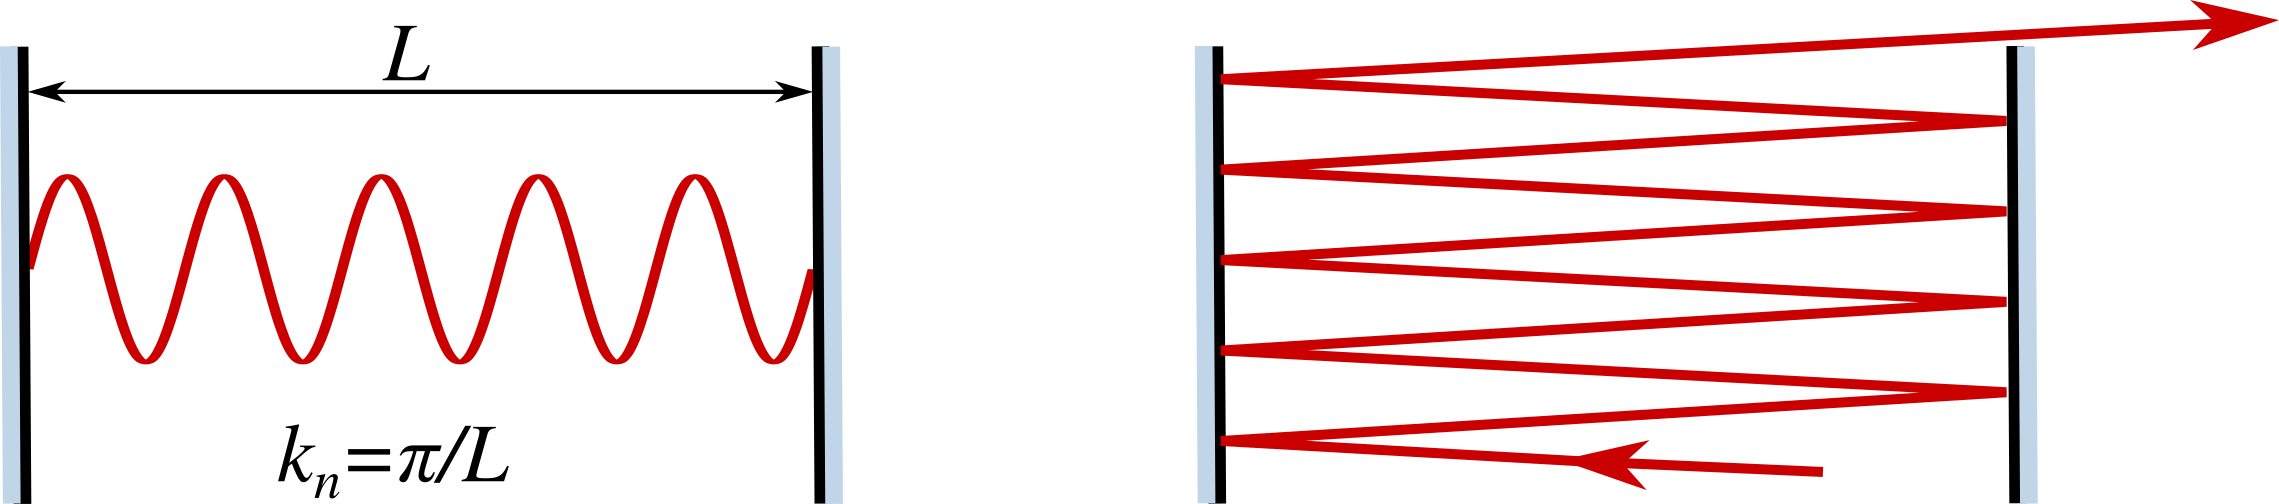
\includegraphics[width=10truecm]{slike/04_Odprt_resonator.png}
\caption{Odprt resonator. Levo: lastni nihajni načini takega resonatorja imajo 
diskretne vrednosti valovnih vektorjev $k_{n}$. Desno: žarki, ki niso pravokotni na ravna zrcala
resonatorja (Fabry-Perotov interferometer) uidejo iz resonatorja.}
\label{fig:Odprt_resonator}
\end{figure}

Oglejmo si odprte resonatorje podrobneje. V zaprti pravokotni votlini velikosti
$a\times a\times L$ z idealno prevodnimi (zrcalnimi) stenami so dovoljene vrednosti
valovnega vektorja za lastna nihanja 
\begin{equation}
\mathbf{k}_{l,m,n}=\left(\frac{l\pi}{a}\,,\frac{m\pi}{a}\,,\frac{n\pi}{L}\right),\label{eq:k-votlina}
\end{equation}
 kjer so $l$, $m$ in $n$ cela števila, $L$ dolžina, $a$ pa prečna
dimenzija resonatorja. Lastne frekvence so 
\begin{equation}
\omega_{l,m,n}=c|\mathbf{k}_{l,m,n}|.\label{eq:omega-votlina}
\end{equation}
Dolžina resonatorja $L$ je velika v primeri z $\lambda$ in zato je $n$
veliko število. Če prečnih sten ni, mora biti $\mathbf{k}$ približno
vzporeden z osjo $z$, zato morata biti $l$ in $m$ majhna. Tedaj
lahko velikost valovnega vektorja razvijemo in dobimo za frekvenco
\begin{equation}
\omega_{l,m,n}=c\left(\frac{n\pi}{L}+\frac{l^{2}+m^{2}}{2n}\frac{L \pi}{a^{2}}\right).
\label{eq:delta-omega-resonator-razvoj}
\end{equation}
Drugi člen v oklepaju je običajno le majhen popravek, tako da so
lastne frekvence odprtih optičnih resonatorjev odvisne predvsem od
števila vozlov v vzdolžni smeri. To je navadno veliko, med $10^{5}$
in $10^{7}$. Možna so tudi lastna nihanja z nekaj vozli v prečni
smeri, ki pa le malo vplivajo na lastne frekvence. Zato bomo v nadaljevanju
obravnavali predvsem lastna stanja brez vozlov v prečni smeri, ki
jih bomo označili z enim samim indeksom $n$.

Razlika frekvenc dveh zaporednih lastnih nihanj\index{Lastne frekvence resonatorja} $n$ in $n+1$ je
\boxeq{eq:delta-omega-resonator}{
\Delta\omega_{n}=\frac{\pi c}{L}.
}
Pri dolžini resonatorja $L=30~\centi\metre$ dobimo v frekvenčni
interval $3\cdot10^{9}~\hertz$ sedaj le še $6$ nihanj, ki jih
je brez težav mogoče razločiti.

V zaprtih votlinah s prevodnimi (zrcalnimi) stenami dobimo dobro določena lastna
stanja pri poljubni obliki votline. Pri odprtih resonatorjih to ne velja.
Da dobimo lastna nihanja z majhnimi izgubami, morata
biti izpolnjena dva pogoja:

\begin{enumerate} 
\item Snop geometrijskih žarkov mora ostati po mnogih odbojih ujet med zrcali resonatorja.\\
\item Polmer zrcala mora biti večji od polmera uklonsko razširjenega snopa, ki izhaja iz nasprotnega zrcala. \\
\end{enumerate}

Resonatorjem, ki zadoščajo gornjima pogojema, pravimo stabilni resonatorji\index{Stabilnost resonatorjev}.
Drugi pogoj lahko zapišemo tudi z enačbami, izhajajoč iz enačbe za oceno divergence (enačba~\ref{eq:kot_ocena}):
\begin{equation}
\vartheta = \frac{\lambda}{a_1} < \frac{a_2}{L} \qquad \Rightarrow \qquad
\frac{a_{1}a_{2}}{\lambda L}>1,
\label{eq:Fresnelovo_stevilo}
\end{equation}
kjer sta $a_{1}$ in $a_{2}$ polmera zrcal resonatorja. Izrazu 
$
F = a_{1}a_{2}/\lambda L
$
pravimo Fresnelovo število\index{Fresnelovo število}.

\subsection*{Fabry-Perotov interferometer}
Poglejmo preprost primer resonatorja, omejenega z dvema vzporednima ravnima zrcaloma
z veliko odbojnostjo. Takemu sistemu pravimo \index{Fabry-Perotov 
interferometer}Fabry-Perotov 
interferometer\footnote{Francoska fizika Maurice Paul Auguste Charles Fabry, 1867--1945, in 
Jean-Baptiste Alfred Perot, 1863--1925.}. 
Da nastane med zrcali stoječe valovanje, mora biti razdalja 
med zrcaloma večkratnik polovične valovne dolžine
\beq
L = \frac{n \lambda}{2},
\eeq
kar je enako pogoju za odprt resonator (enačba~\ref{eq:k-votlina}). 

\begin{definition}
Pokaži, da je prepustnost Fabry-Perotovega interferometra, katerega zrcali imata odbojnost $\cal{R}$, enaka 
\beq
T = \frac{1}{1+\frac{4\cal{R}}{(1-{\cal R})^2}\sin^2 \delta},
\eeq
kjer je $\delta = kL\cos{\vartheta}$, $L$ razmik med zrcaloma, $\vartheta$ vpadni kot, 
$k$ pa valovni vektor svetlobe.
\end{definition}

Prepustnost interferometra za ravni val, ki vpada pravokotno na zrcala z
odbojnostjo ${\cal R}$, je 
\begin{equation}
T=\frac{1}{1+\frac{4{\cal R}}{(1-{\cal R})^{2}}\sin^{2}kL}
\label{eq:Fabry-Perot-prepustnost}
\end{equation}
in je prikazana na sliki (\ref{fig:Fabry-Perot}).
Ko je frekvenca vpadnega valovanja ravno enaka lastni frekvenci
resonatorja, je sistem v resonanci in  $T=1$. Širina resonance je tem manjša, čim
večja je odbojnostjo zrcal. Ta seveda tudi določa čas dušenja vzbujenega
lastnega nihanja.\\
\begin{figure}[h]
\centering
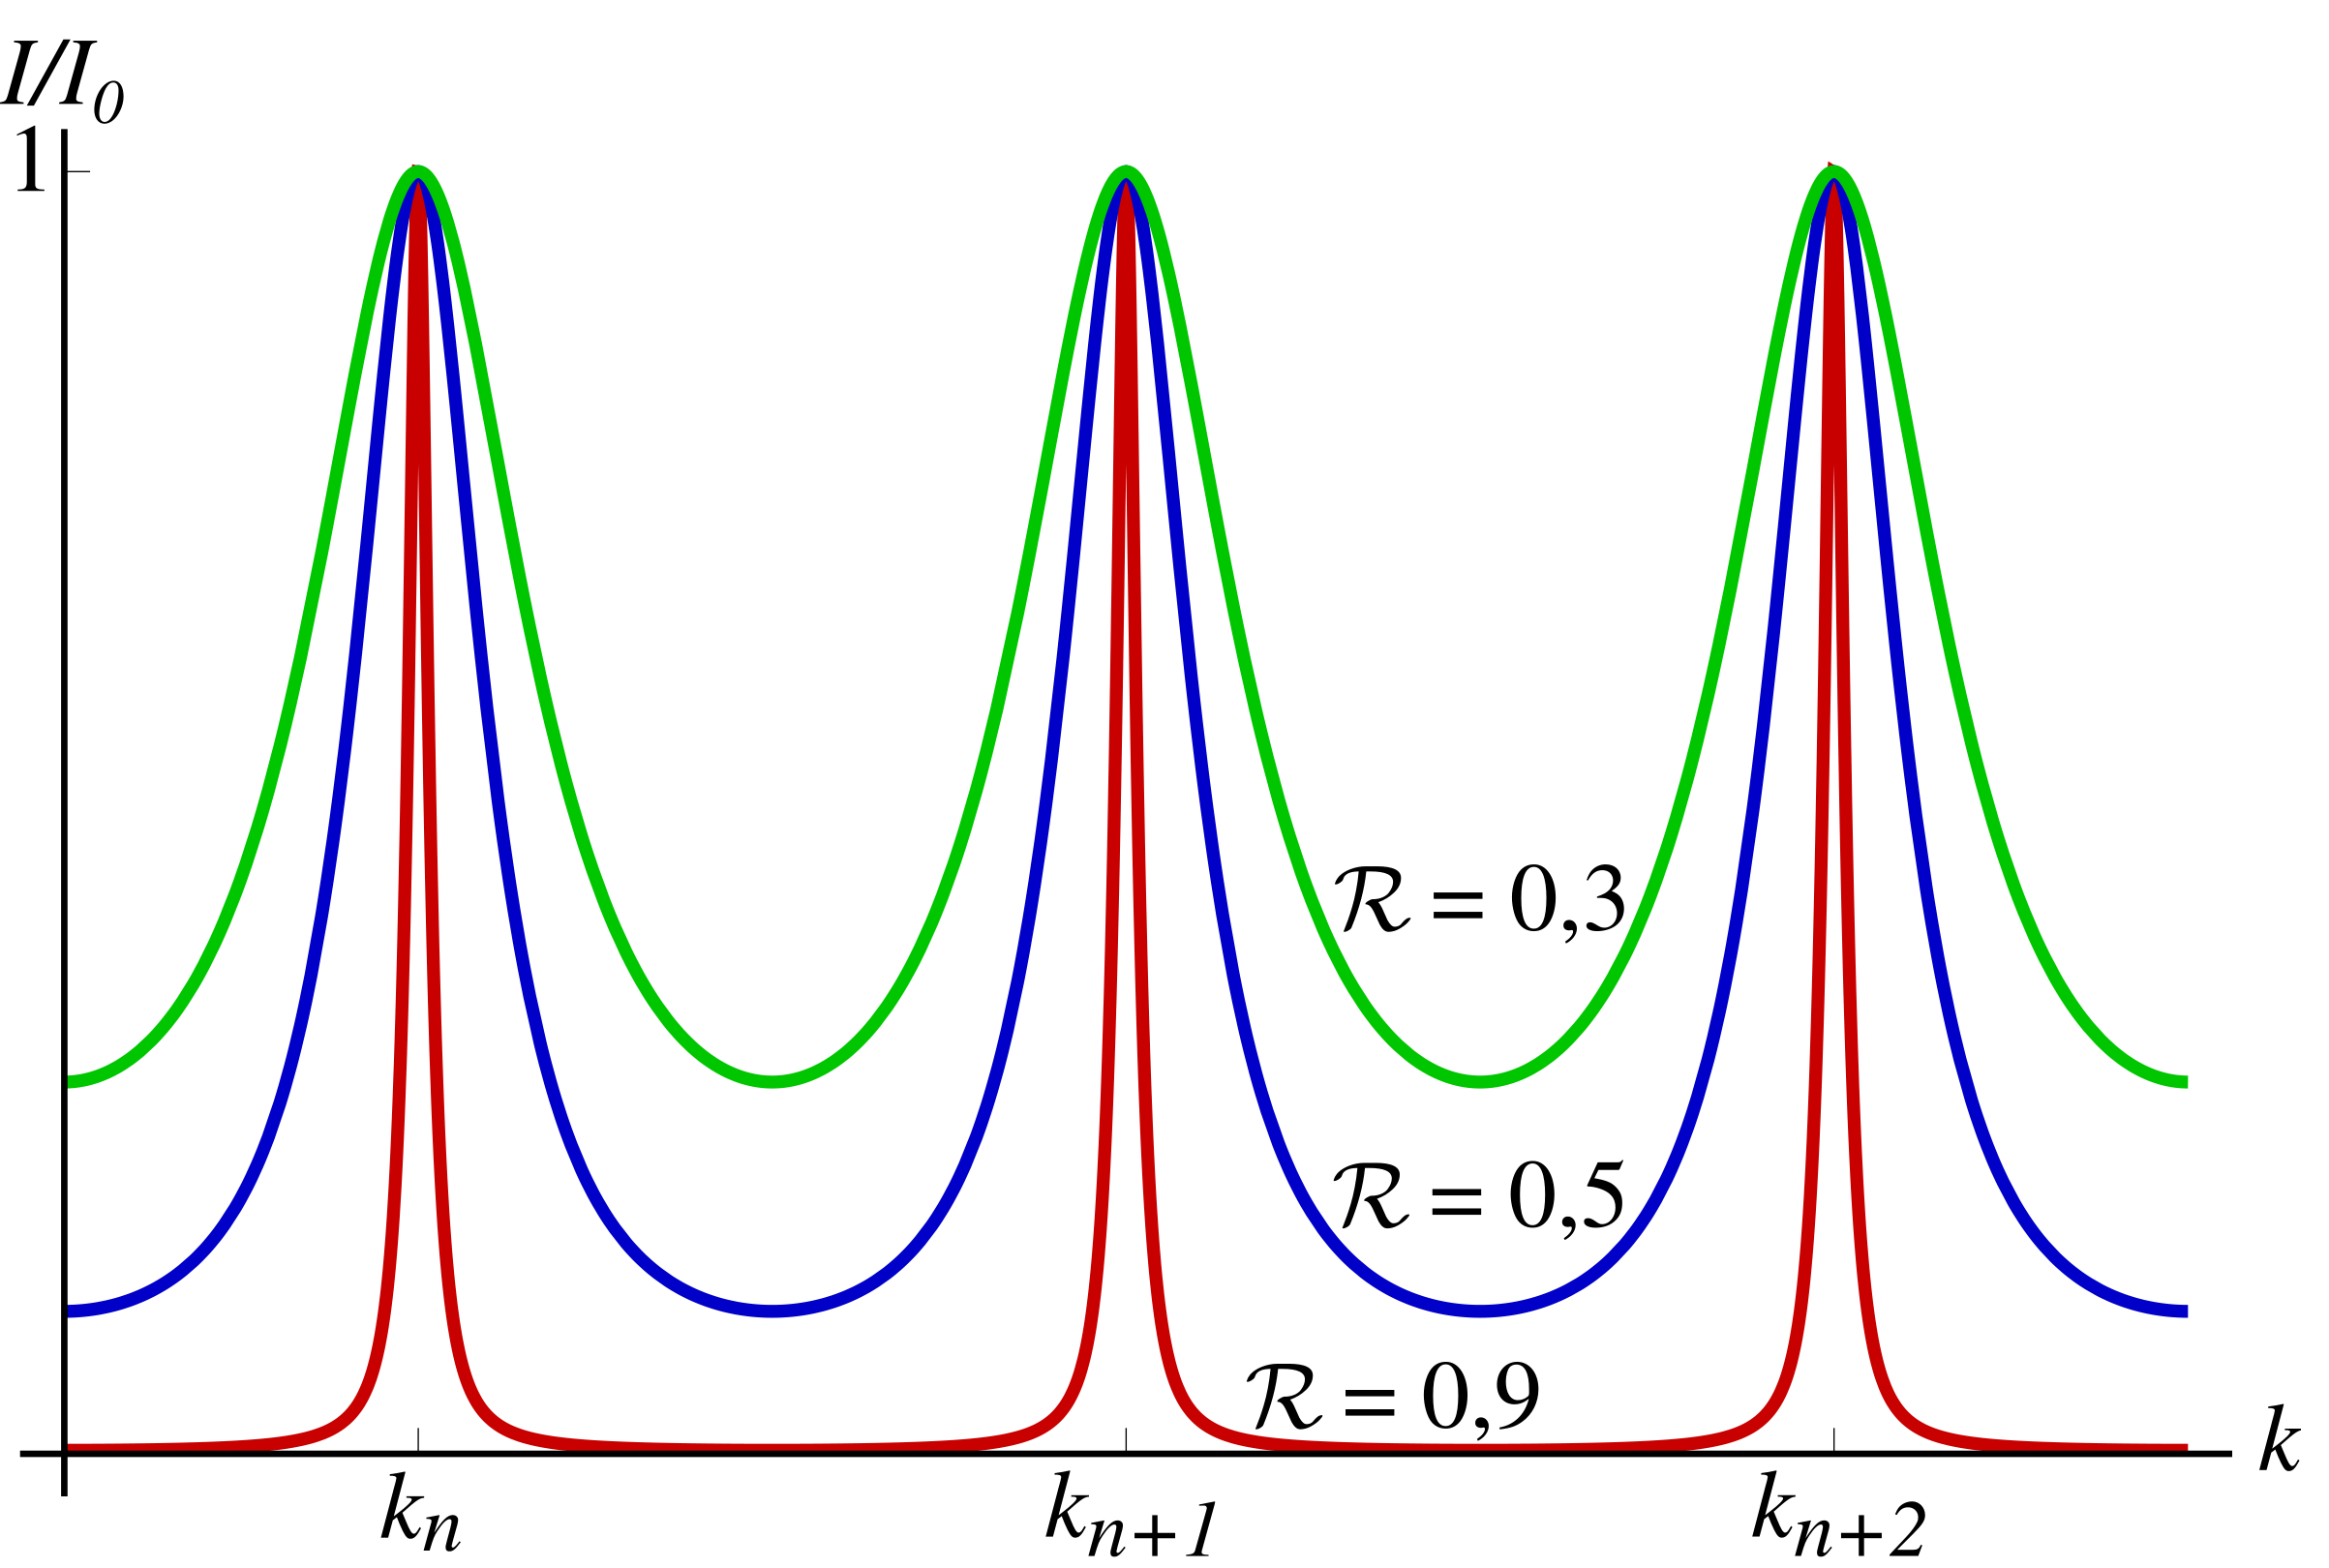
\includegraphics[width=9truecm]{slike/04_fabry_perot.png}
\caption{
Prepustnost Fabry-Perotovega interferometra
v odvisnosti od valovnega vektorja $k$ za tri različne odbojnosti zrcal
$\mathcal{R}.$}
\label{fig:Fabry-Perot}
\end{figure}

Prvemu pogoju stabilnosti ustrezajo v Fabry-Perotovem interferometru
le žarki, ki so natanko pravokotni na zrcali. Čim sta zrcali le
malo nevzporedni, stabilnih žarkov sploh ni več. Tako imenovani planparalelni 
interferometer\index{Resonator!planparalelni} je tako na meji stabilnosti. Z izpolnjevanjem drugega
pogoja ni težav, saj morajo biti pri na primer $30~\centi\metre$ dolgem resonatorju in 
valovni dolžini $0,5~\mu\metre$ zrcala večja od $0,4~\milli\metre$, da zadostijo pogoju, 
zapisanem v enačbi~(\ref{eq:Fresnelovo_stevilo}).

Bolj stabilne resonatorje lahko dobimo, če vzamemo par konkavno ukrivljenih
zrcal. Tedaj so žarki, ki potujejo pod majhnim kotom glede na osrednjo os, ujeti
med zrcali in energija lastnih valovanj ostaja lokalizirana blizu
osi.

\section{Gaussovi snopi v resonatorjih}
V stabilnih resonatorjih s konkavnimi zrcali pričakujemo, da so
lastna valovanja omejena na bližino osrednje osi. Zrcala so tako mnogo 
večja od polmera lastnega nihanja. Tedaj lahko za obravnavo
električnega polja uporabimo obosno valovno enačbo (enačba~\ref{eq:obosna-valovna-enacba}). 
Veliko odbojnost na zrcalih dobimo tedaj, kadar je njihova električna prevodnost velika. 
Iz tega izhaja robni pogoj, ki pravi, da je električno polje na zrcalu 
približno nič. Valovna fronta stoječega valovanja na zrcalu mora zato 
sovpadati s površino zrcala.

\begin{figure}[h]
\centering
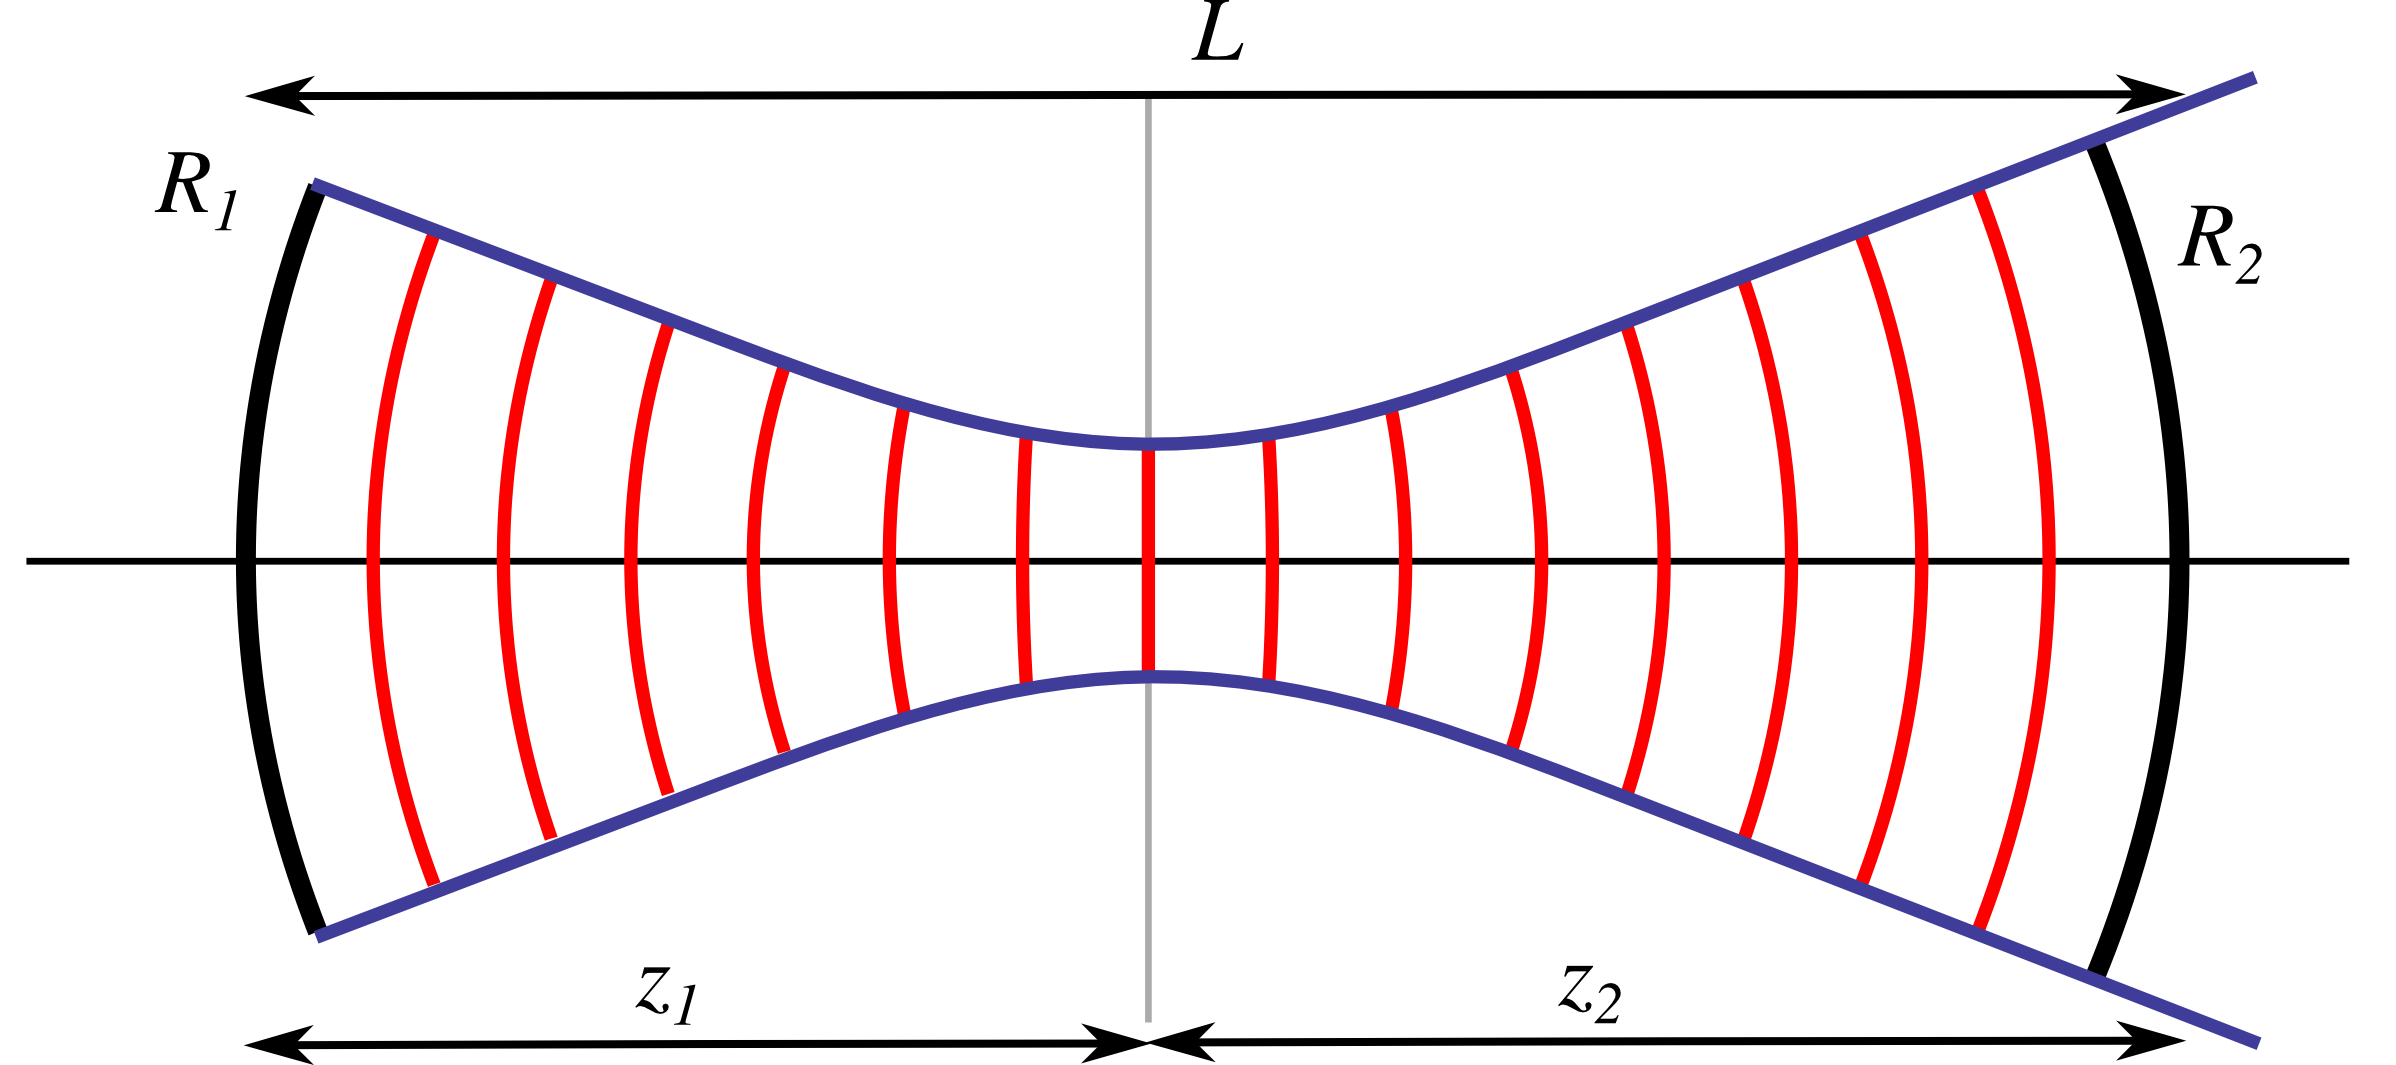
\includegraphics[width=11truecm]{slike/04_Resonator_Gauss.png}
\caption{Gaussov snop v odprtem resonatorju s konkavno ukrivljenimi zrcali. 
Krivinski radij zrcal se ujema s krivinskim radijem čela snopa.}
\label{fig:Gaussov-snop-v-resonatorju}
\end{figure}

V prečni smeri omejene rešitve obosne enačbe smo našli v obliki potujočih
Gaussovih snopov\index{Gaussov snop}. Podobno kot zapišemo stoječe valovanje na vrvi, 
lahko stoječe snope dobimo s superpozicijo snopov, ki se širijo v različnih smereh ob osi. 
Da zadostimo robnim pogojem na zrcalih, se mora krivinski radij snopa ujemati s
krivinskima radijema zrcal $R_{1}$ in $R_{2}$ (slika \ref{fig:Gaussov-snop-v-resonatorju}).
Pri tem sta neznanki polmer grla snopa, ki je podan s parametrom $z_{0}$,
in lega grla. Postavimo izhodišče osi $z$ v grlo, kot smo
navajeni, tako da sta zrcali pri $z_{1}<0$ in $z_{2}>0$. Z uporabo enačbe
za krivinski radij snopa $R$ (enačba~\ref{eq:R}) dobimo 
\begin{eqnarray}
-R_{1} & = & z_{1}\left[1+\left(\frac{z_{0}}{z_{1}}\right)^{2}\right] \quad \textrm{in}\\
R_{2} & = & z_{2}\left[1+\left(\frac{z_{0}}{z_{2}}\right)^{2}\right].
\label{eq:krivinski}
\end{eqnarray}
Pri tem smo upoštevali, da je krivinski radij za konkavno zrcalo glede na pozitivno smer $z$ pozitiven.
Veljati mora še 
\begin{equation}
z_{2}-z_{1}=L
\label{eq:razlikaz}
\end{equation}
Iz gornjih enačb najprej izračunamo razdaljo $z_{1}$, ki določa
položaj grla v resonatorju, nato pa parameter $z_{0}$, ki določa
območje bližnjega polja in preko enačbe~(\ref{eq:z0}) enolično tudi polmer grla: 
\begin{equation}
z_{0}^{2}=\frac{L(R_{1}-L)(R_{2}-L)(R_{1}+R_{2}-L)}{(R_{1}+R_{2}-2L)^{2}}.
\label{eq:z0_stab}
\end{equation}
Da je snop realen in omejen, mora biti $z_{0}^{2}>0$ in zato števec
gornjega izraza pozitiven. Ta pogoj lahko po kratkem računu zapišemo
v obliki stabilnostnega kriterija\index{Stabilnostni kriterij}
\boxeq{eq:stabilnost}{
0<\left(1-\frac{L}{R_{1}}\right)\left(1-\frac{L}{R_{2}}\right)<1.
}
Resonatorji, ki zadoščajo gornjemu pogoju, so stabilni. 

\begin{definition}
Izhajajoč iz enačb~(\ref{eq:krivinski}) in (\ref{eq:razlikaz}) izpelji 
kriterij za stabilnost resonatorja
(enačba~\ref{eq:stabilnost}).
\end{definition}

Stabilnostni kriterij za resonatorje je najbolj nazorno predstaviti na diagramu, 
kjer na os $x$ nanašamo $L/R_{1}$ in na os $y$ $L/R_{2}$. Na 
sliki~(\ref{fig:Podrocje-stabilnih-resonatorjev}) je stabilno območje delovanja 
resonatorjev, kot ga razberemo iz enačbe~(\ref{eq:stabilnost}), označeno senčeno.
Opazimo, da je možno veliko različnih tipov stabilnih resonatorjev, ob tem da 
resonatorji, ki so sestavljeni iz dveh konveksnih zrcal, niso nikoli stabilni.
Če je eno zrcalo ravno (plankonkavni resonatorji), je grlo Gaussovega snopa vedno 
na ravnem zrcalu. V primeru konveksno-konkavnega resonatorja leži grlo snopa
izven resonatorja. Podrobneje si oglejmo nekaj posebnih primerov stabilnih resonatorjev. 

\begin{figure}[h]
\centering
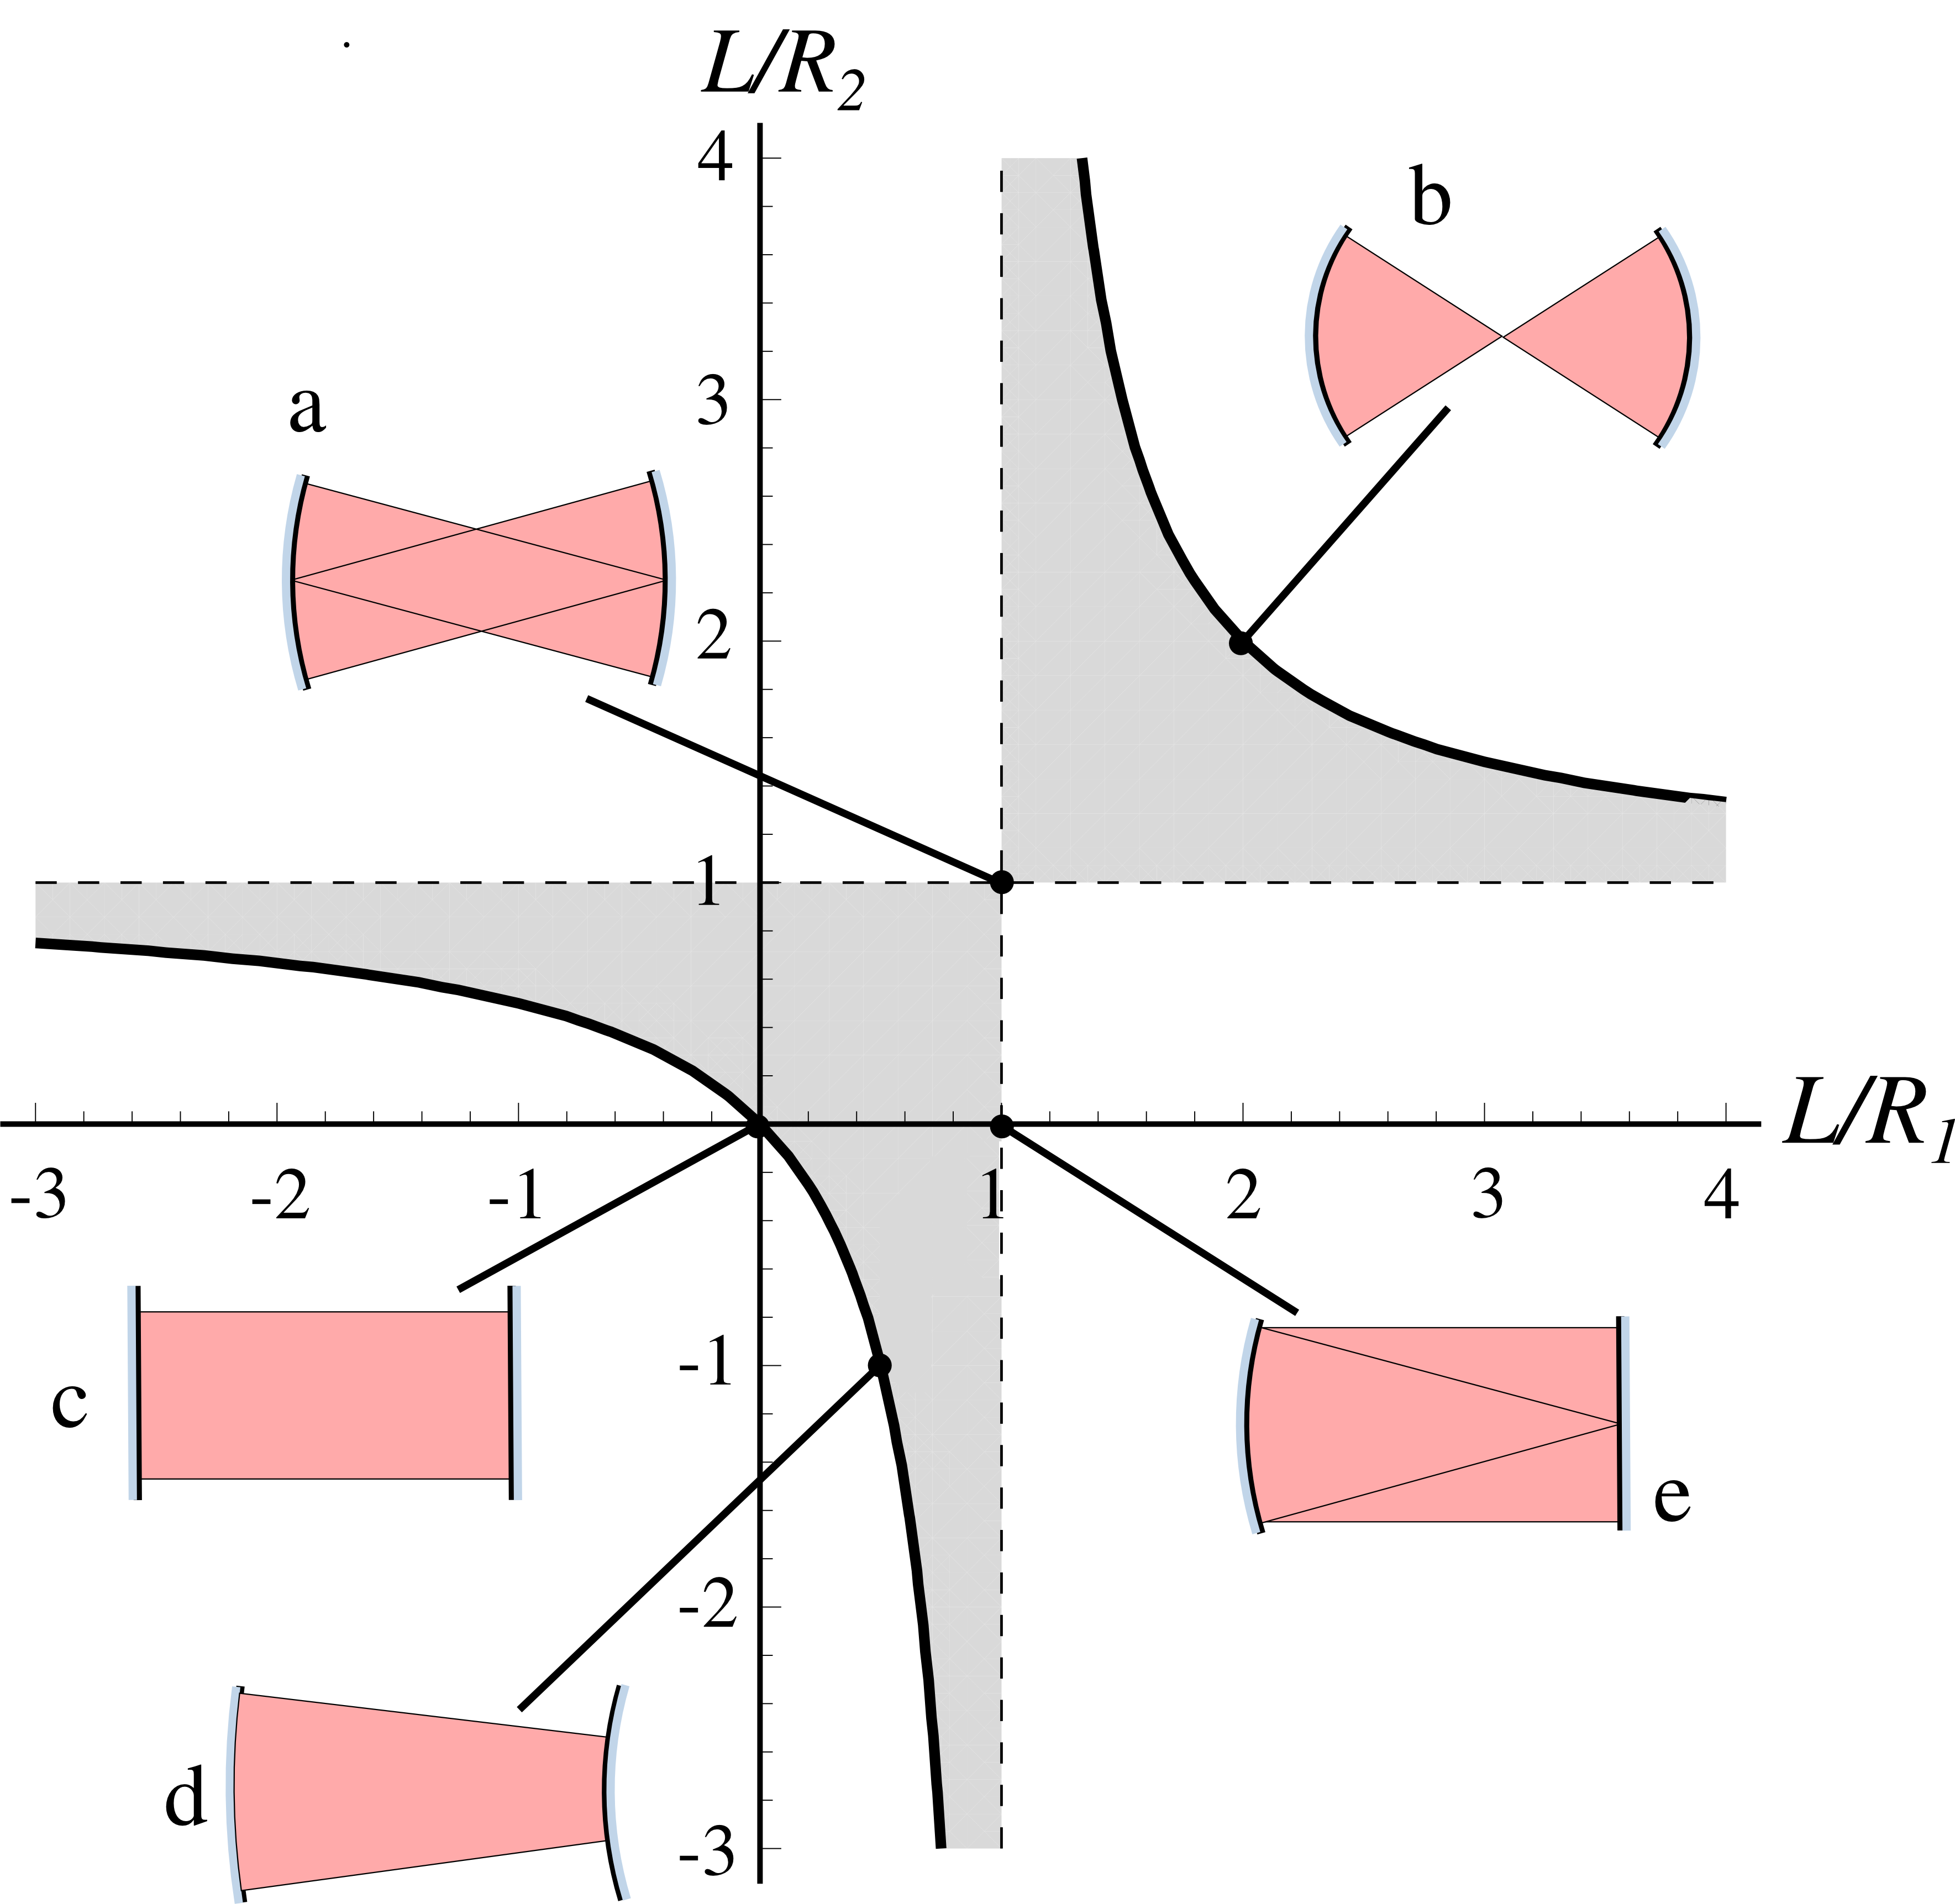
\includegraphics[width=8truecm]{slike/04_Stabilnost.png}
\caption{Področje stabilnih resonatorjev. Resonator je stabilen, 
če sta parametra $L/R_{1}$ in $L/R_{2}$ znotraj osenčenega območja. (a) konfokalni resonator,
(b) koncentrični resonator, (c) planparalelni resonator (Fabry-Perot), 
(d) konveksno-konkavni resonator in (e) plankonkavni resonator.}
\label{fig:Podrocje-stabilnih-resonatorjev}
\end{figure}

\subsection*{Simetrični resonatorji}
Za simetrični resonator\index{Resonator!simetrični} velja $R_{1}=R_{2}=R$. Na diagramu 
(slika~\ref{fig:Podrocje-stabilnih-resonatorjev}) 
se taki resonatorji nahajajo na simetrali lihih kvadrantov, $x=y$. Pri simetričnih resonatorjih 
je grlo v sredini resonatorja in enačba~(\ref{eq:stabilnost}) se poenostavi v 
\begin{equation}
z_{0}=\frac{1}{2}\sqrt{(2R-L)L}.
\label{eq:zosim}
\end{equation}
Polmer grla v simetričnem resonatorju je enak
\begin{equation}
w_{0}=\sqrt{\frac{\lambda z_{0}}{\pi}}=\sqrt{\frac{\lambda}{2\pi}}\sqrt[4]{(2R-L)L}.
\label{eq:grlo_v_res}
\end{equation}
Po enačbi~(\ref{eq:w}) lahko izračunamo še polmer snopa na ogledalu
\begin{equation}
w_{1}^{2}=w_{0}^{2}\left[1+\left(\frac{L}{2z_{0}}\right)^{2}\right]=
\frac{\lambda}{\pi}\frac{R\sqrt{L}}{\sqrt{2R-L}}
\end{equation}

Pri dani dolžini simetričnega resonatorja je polmer snopa na zrcalu najmanjši,
kadar je $R=L$. Tedaj sovpadata geometrijski gorišči obeh zrcal,
zato imenujemo tak resonator konfokalni\index{Resonator!konfokalni}. 
Hiter račun pokaže, da velja $z_{0}=L/2$, snop od grla do zrcala pa se razširi
za $w_1/w_0=\sqrt{2}$. 
\begin{definition}
\label{naloga:uklon_konf}
 Pokaži, da je polmer snopa na izhodnem zrcalu v simetričnem resonatorju s parametri $R,L$
 najmanjši, kadar je resonator konfokalni.
\end{definition}

Pri načrtovanju laserjev pa imamo dodatno omejitev, saj moramo poskrbeti za 
čim boljšo izrabo ojačevalnega sredstva. Pogosto je zato 
polmer grla snopa razmeroma velik. Iz enačbe~(\ref{eq:grlo_v_res})
sledi, da mora biti v tem primeru krivinski radij zrcal velik. S tem
pridobimo na ojačanju, po drugi strani pa se nekoliko poslabša stabilnost.

Poglejmo primer. Naj bo dolžina resonatorja He-Ne laserja $L=1~\metre$ in valovna
dolžina $\lambda = 633$~nm. Tedaj je v konfokalni geometriji po enačbi~(\ref{eq:grlo_v_res})
polmer grla $w_{0}=0,32$~mm. Premer razelektritvene cevi je običajno
nekaj milimetrov in približno tako debel mora biti tudi svetlobni
snop, če naj dobro izkoristi ojačanje zaradi stimuliranega sevanja.
Da bi pri isti dolžini laserja dobili grlo s premerom 2~mm, moramo vzeti
zrcala s krivinskim radijem okoli 50~m. Primer kaže, da že majhna ukrivljenost 
zrcal zagotovi dokaj ozke snope.

\begin{remark}
Izkaže se, da so konfokalni resonatorji najmanj občutljivi na majhne zasuke enega zrcala. 
Pri zasuku zrcala se v navadnih stabilnih resonatorjih namreč premakne os, ki gre skozi 
krivinski središči obeh zrcal. Če želimo, da je največji odmik nove osi čim
manjši, uporabimo konfokalne resonatorje. 
\end{remark}

Skrajna primera stabilnega simetričnega resonatorja sta 
koncentrični resonator\index{Resonator!koncentrični},
pri katerem sovpadata krivinski središči zrcal in $L=2R$, in planparalelni 
resonator\index{Resonator!planparalelni}, pri katerem sta zrcali ravni $R \to \infty$.
V prvem primeru gre po enačbi~(\ref{eq:grlo_v_res}) polmer grla proti nič, v drugem pa raste sorazmerno
z $R^{1/4}$. Pri povsem ravnih ogledalih postanejo uklonske
izgube na robovih ogledal znatne. Račun z Gaussovimi snopi tedaj ni več veljaven
in treba je uporabiti druge pristope, ki jih bomo na kratko opisali
v razdelku~(\ref{Resonator_uklon}).

V prejšnjem poglavju smo videli, da obstajajo poleg osnovnega Gaussovega
snopa še rešitve obosne enačbe z vozli v prečni smeri, to je snopi
višjega reda. Imajo enak parameter $z_{0}$ in enako ukrivljenost
valovnih ploskev, zato so seveda tudi dobre rešitve za polje v stabilnih
resonatorjih. Pri tem je treba vedeti, da je pri enakem $w_{0}$
dejanski polmer snopa reda $n$ za približen faktor $\sqrt{n}$ večji 
(glej nalogo~\ref{naloga:HG}). Če želimo dobiti iz laserja samo 
osnovni Gaussov snop (imenovan tudi $TEM_{00}$), ki ima od vseh snopov
najbolj gladko valovno fronto, ohranja prečno obliko in ima najmanjšo 
divergenco pri danem polmeru grla, pogosto uporabimo zaslonko
ustrezne velikosti, ki snope višjih redov poreže, ali kakšen drug
element, na primer Fabry-Perotov etalon, ki poveča izgube za snope višjega reda.
 
\begin{remark}
V praksi se včasih uporabljajo tudi nestabilni resonatorji, to je
taki, za katere ne obstojajo rešitve v obliki Gaussovih snopov. Taki
resonatorji imajo velike izgube na robovih zrcal, ker žarki v njih niso ujeti. 
Uporabni so v laserjih z velikim ojačanjem. Njihova prednost je, da je cel
volumen resonatorja enakomerno pokrit s svetlobo.
\end{remark}

\section{Stabilnostni kriterij z ABCD formalizmom}
V prejšnjem razdelku smo izpeljali pogoj za stabilnost resonatorja, 
sestavljenega iz dveh zrcal s polmeroma $R_1$ in $R_2$, ki sta med 
seboj oddaljeni za $L$. Izhajali smo iz pogoja, da se ukrivljenost
valovnih front na zrcalu ujema z ukrivljenostjo zrcal. Vendar so sistemi,
kjer imamo zgolj dve zrcali, razmeroma redki. Pogosto so v resonatorju
druge optične komponente, ki jih je treba upoštevati pri zapisu
kriterija za stabilnost. Takrat si pomagamo z matrikami ABCD\index{ABCD matrike}. Poglejmo, kako.

Izhajajmo iz trditve, da se v stabilnem resonatorju snop po enem celotnem obhodu
preslika sam vase. Gaussov snop na neki točki v resonatorju 
zapišemo s kompleksno ukrivljenostjo (enačba~\ref{eq:q-inv})
\beq
\frac{1}{q}= \frac{1}{R(z)}+i\frac{2}{kw(z)^{2}}.
\eeq
V najpreprostejšem primeru resonatorja snop prepotuje dano razdaljo, se odbije od zrcala, prepotuje
resonator v nasprotni smeri, se odbije od drugega zrcala in se vrne v začetno lego. V bolj 
zapletenih primerih dodamo še prehode skozi druge optične elemente. Matriko 
za celotni prehod potem zapišemo kot produkt matrik ABCD za posamezne prehode $M = M_N M_{N-1} ...M_2 M_1$.
Končni produkt za celoten obhod je matrika oblike
\beq
M = \left[\begin{array}{cc}
A & B\\
C & D
\end{array}\right],
\eeq
kompleksni krivinski radij po prehodu pa je enak začetnemu kompleksnemu radiju
\beq
q_2 = \frac{Aq+B}{Cq+D} = q.
\eeq
Gornjo enačbo prepišemo v 
\beq
Cq^2+(D-A)q-B=0.
\eeq
Ker mora biti $q$ kompleksen, da dobimo realno vrednost $w$, mora biti diskriminanta
kvadratne enačbe negativna
\beq
(D-A)^2+ 4BC<0.
\eeq
Upoštevamo še, da je determinanta matrike $AD-BC=1$ in dobimo pogoj za 
stabilnost\index{Stabilnostni kriterij}, zapisan s koeficienti matrike $M$:
\boxeq{eq:stabilnost_ABCD}{
-1 < \left(\frac{A+D}{2}\right) < 1.
}

\begin{definition}
Pokaži, da je za resonator z dolžino $L$ in s konkavnima zrcaloma ($R_1$ in $R_2$) 
pogoj za stabilnost (enačba~\ref{eq:stabilnost_ABCD}) ekvivalenten pogoju~(\ref{eq:stabilnost}).
\end{definition}

Podoben, a malo bolj zapleten račun lahko naredimo tudi za resonatorje, v katerih se snop 
ne vrne v svojo začetno obliko po enem obhodu, ampak je teh obhodov $n$. Potem zapišemo
matriko $M$ kot produkt elementov v enem obhodu, celotna matrika pa je enaka $M^n$. Iz pogoja,
da matrika ne divergira za velike $n$, dobimo pogoj za stabilnost, ki je natančno 
enak pogoju~(\ref{eq:stabilnost_ABCD}), ki smo ga ravnokar izpeljali. 

\section{Resonančne frekvence}
Doslej smo obravnavali le prostorsko obliko polja v resonatorju, ničesar pa še nismo
povedali o časovni odvisnosti lastnih nihanj. Frekvence
lastnih nihanj\index{Lastne frekvence resonatorja} dobimo iz pogoja, da se mora faza snopa pri enem obhodu,
to je pri preletu resonatorja v obeh smereh, spremeniti za mnogokratnik
$2\pi$. Fazo za osnovni snop zapišemo po enačbi~(\ref{eq:gaussov-snop})\index{Gouyeva faza}
\begin{equation}
kz+\frac{kr^{2}}{2R} -\eta(z) = kz-\arctan \left(\frac{z}{z_{0}}\right),
\label{eq:fazag}
\end{equation}
pri čemer smo upoštevali, da gledamo valovanje na osi, pri $r=0$. 
Resonančni pogoj je, da je razlika te faze pri prehodu od enega zrcala
do drugega mnogokratnik $\pi$: 
\begin{equation}
\frac{\omega_{n}}{c}L-\left[\arctan \left(\frac{z_{2}}{z_{0}}\right)-
\arctan\left(\frac{z_{1}}{z_{0}}\right)\right]=n\pi
\label{eq:fazan}
\end{equation}
Pri tem smo zanemarili, da lahko pride do dodatne majhne spremembe
faze pri odboju na zrcalu. Ta za delček valovne dolžine
spremeni efektivno dolžino resonatorja, ki je navadno niti ne poznamo
tako natančno. Iz istega razloga nam ni treba upoštevati člena
v oglatem oklepaju enačbe~(\ref{eq:fazan}), kadar imamo opravka le z osnovnim
snopom. Zanj tako dobimo znano enačbo za resonančne frekvence 
\begin{equation}
\omega_{n}=\frac{n\pi c}{L}.
\label{eq:omega}
\end{equation}
Razmik med dvema zaporednima lastnima frekvencama je 
\begin{equation}
\Delta\omega=\frac{\pi c}{L},
\label{eq:deltaomega}
\end{equation}
kar je v skladu z enačbo~(\ref{eq:delta-omega-resonator}). 

Za snope višjega reda, ki imajo vozle v prečni smeri, je fazni premik
odvisen tudi od števila vozlov. Tako je na primer v cilindričnih koordinatah
(enačba~\ref{eq:etaGL})
\begin{equation}
\eta_{p,l}(z)=(2p+l+1)\arctan\left(\frac{z}{z_{0}}\right)
\end{equation}
in resonančni pogoj zapišemo kot
\begin{equation}
\frac{\omega_{n,p,l}}{c}L-(2p+l+1)\left[\arctan\left(\frac{z_{2}}{z_{0}}\right)-
\arctan\left(\frac{z_{1}}{z_{0}}\right)\right]=n\pi.
\end{equation}
Resonančne frekvence so torej odvisne tudi od števila prečnih vozlov,
kar je dodaten razlog, da v laserjih vzbujamo le osnovno lastno nihanje.

Zanimiv in praktično pomemben je primer konfokalnega resonatorja\index{Resonator!konfokalni},
pri katerem je $z_{0}=L/2$ in $\arctan(L/2z_{0})= \arctan(1)=\pi/4$. Resonančne frekvence
so 
\begin{equation}
\omega_{n,p,l}=\frac{\pi c}{L}\left[n+\frac{1}{2}(2p+l+1)\right].
\label{eq:omega_konf}
\end{equation}

Za snope, pri katerih je $2p+l$ liho število, dobimo iste resonančne frekvence kot
za osnovne snope, pri sodih $2p+l$ pa dobimo še resonance na sredini
med osnovnimi. Razmik med sosednjimi frekvencami je tako $\Delta\nu=c/4L$
in konfokalni interferometer se obnaša kot dvakrat daljši planparalelni.
To lahko razumemo tudi iz geometrijske slike: žarek, ki vstopi v konfokalni
interferometer vzporedno z osjo, se šele po dveh preletih vrne sam
vase.

\begin{figure}[h]
\centering
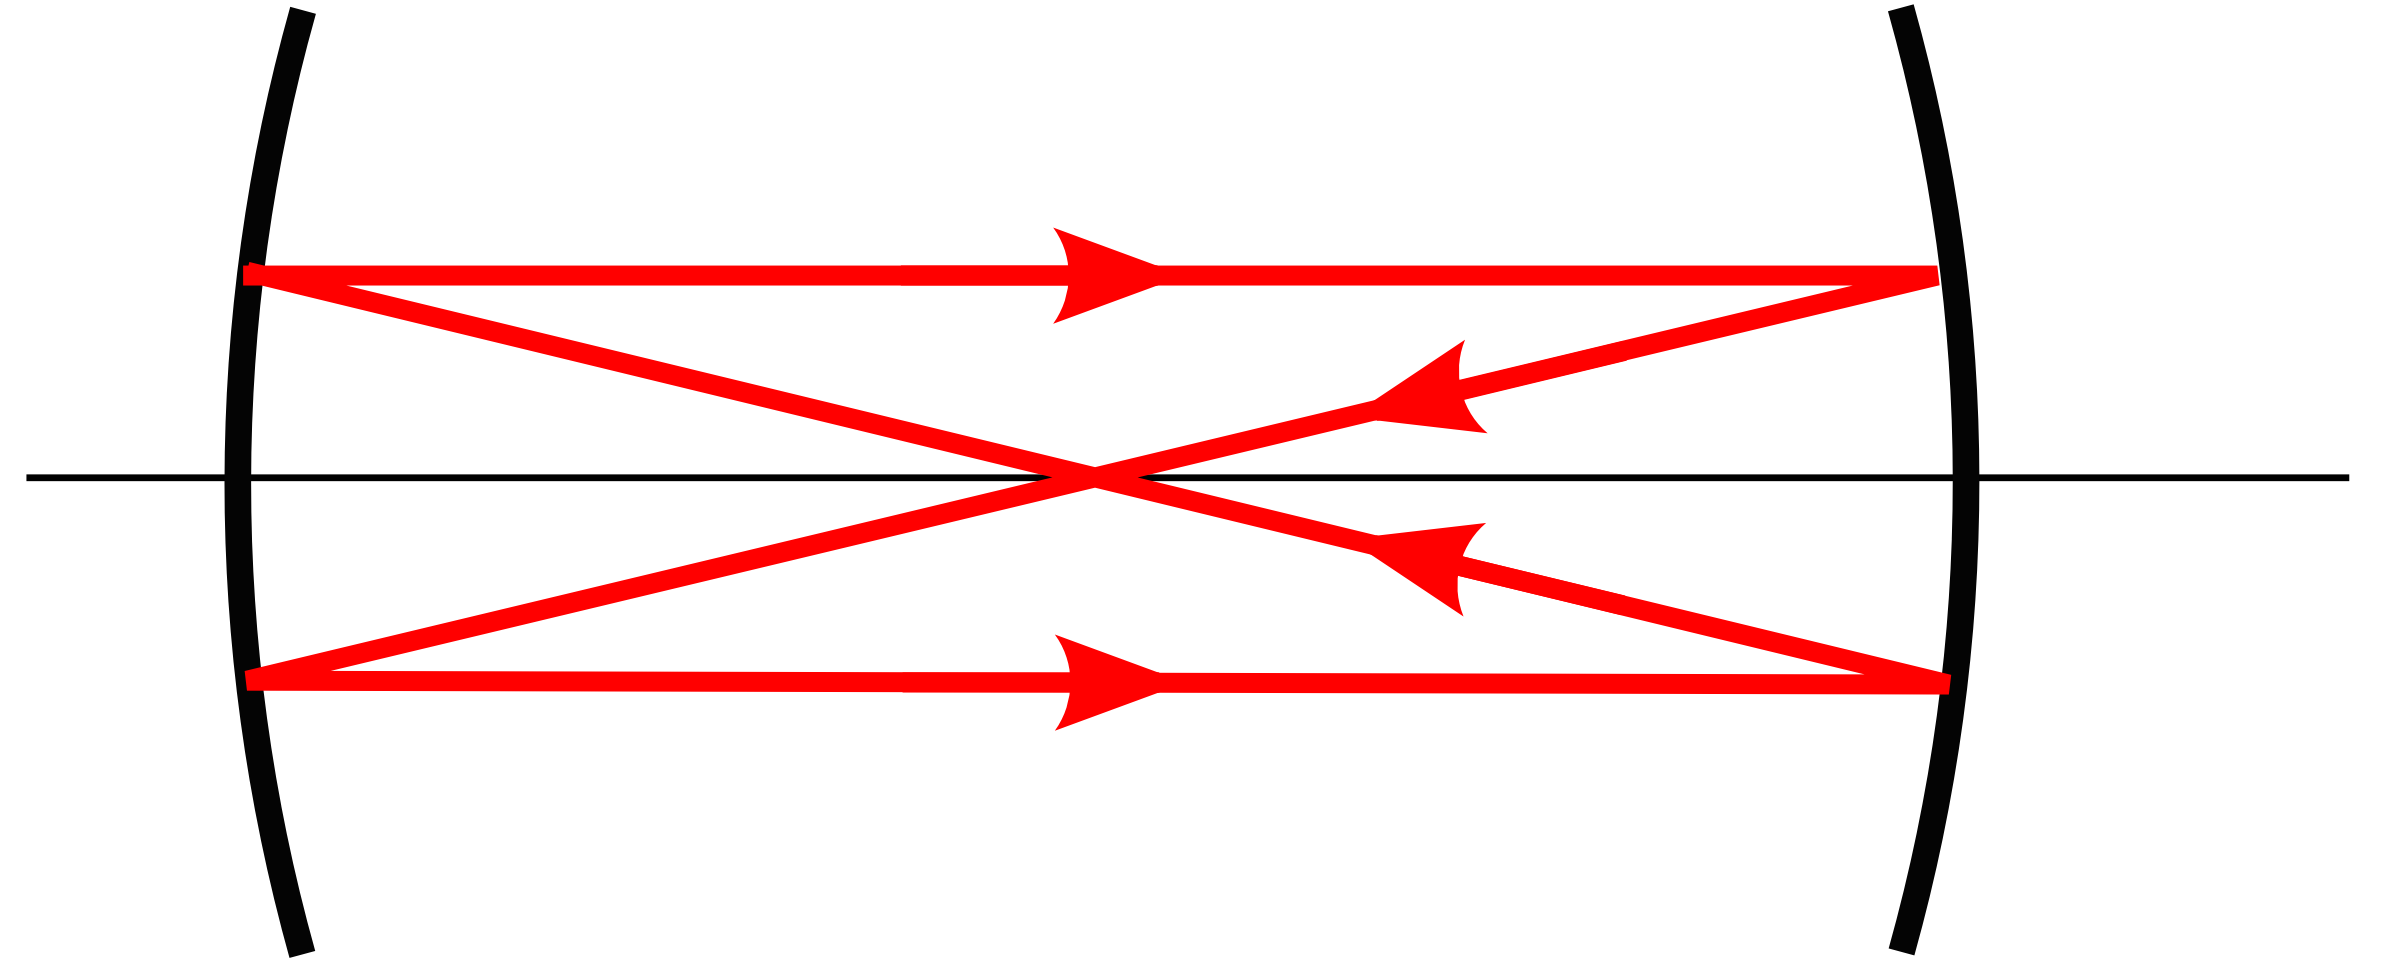
\includegraphics[width=6truecm]{slike/04_Konfokalni.png}
\caption{V konfokalnem resonatorju se žarek šele po dveh preletih
vrne sam vase.}
\label{fig:Konfokalni_zarek}
\end{figure}

V primeru skoraj planparalelnega\index{Resonator!planparalelni} 
resonatorja je $z_{0}\gg L$ in lahko
$\arctan(L/2z_{0})$ razvijemo, upoštevamo enačbo~(\ref{eq:zosim}) in dobimo
\beq
\omega_{n,p,l}=\frac{\pi c}{L}\left[n+(2p+l+1)\frac{1}{\pi}\sqrt{\frac{2L}{R}}\right].
\eeq
Ker je $L$ majhen v primerjavi z $R$, so resonance snopov nizkega prečnega reda 
zelo blizu resonancam osnovnih snopov, niso pa čisto enake. Poglejmo primer. Vzemimo 
simetrični resonator z dolžino $L=1$~m, krivinskim radijem zrcal $R=50$~m, 
valovna dolžina pa naj bo $\lambda= 500$~nm. Z uporabo enačbe~(\ref{eq:zosim})
hitro lahko izračunamo $z_0 = 4,97$~m. Ker je pogoj $z_0\gg L$ izpolnjen, lahko uporabimo
gornji približek. Razlika med frekvencama za dva zaporedna osnovna snopa 
\beq
\Delta \omega_{n,p,l} = \frac{\pi c}{L} = 940~\mathrm{MHz},
\eeq
medtem ko je razlika med frekvencama dveh prečnih snopov
\beq
\Delta \omega_{n,p,l} = \frac{c}{L}\sqrt{\frac{2L}{R}}  = 60~\mathrm{MHz}.
\eeq
Skica spektra lastnih frekvenc je na sliki~(\ref{fig:crte})
\begin{figure}[h]
\centering
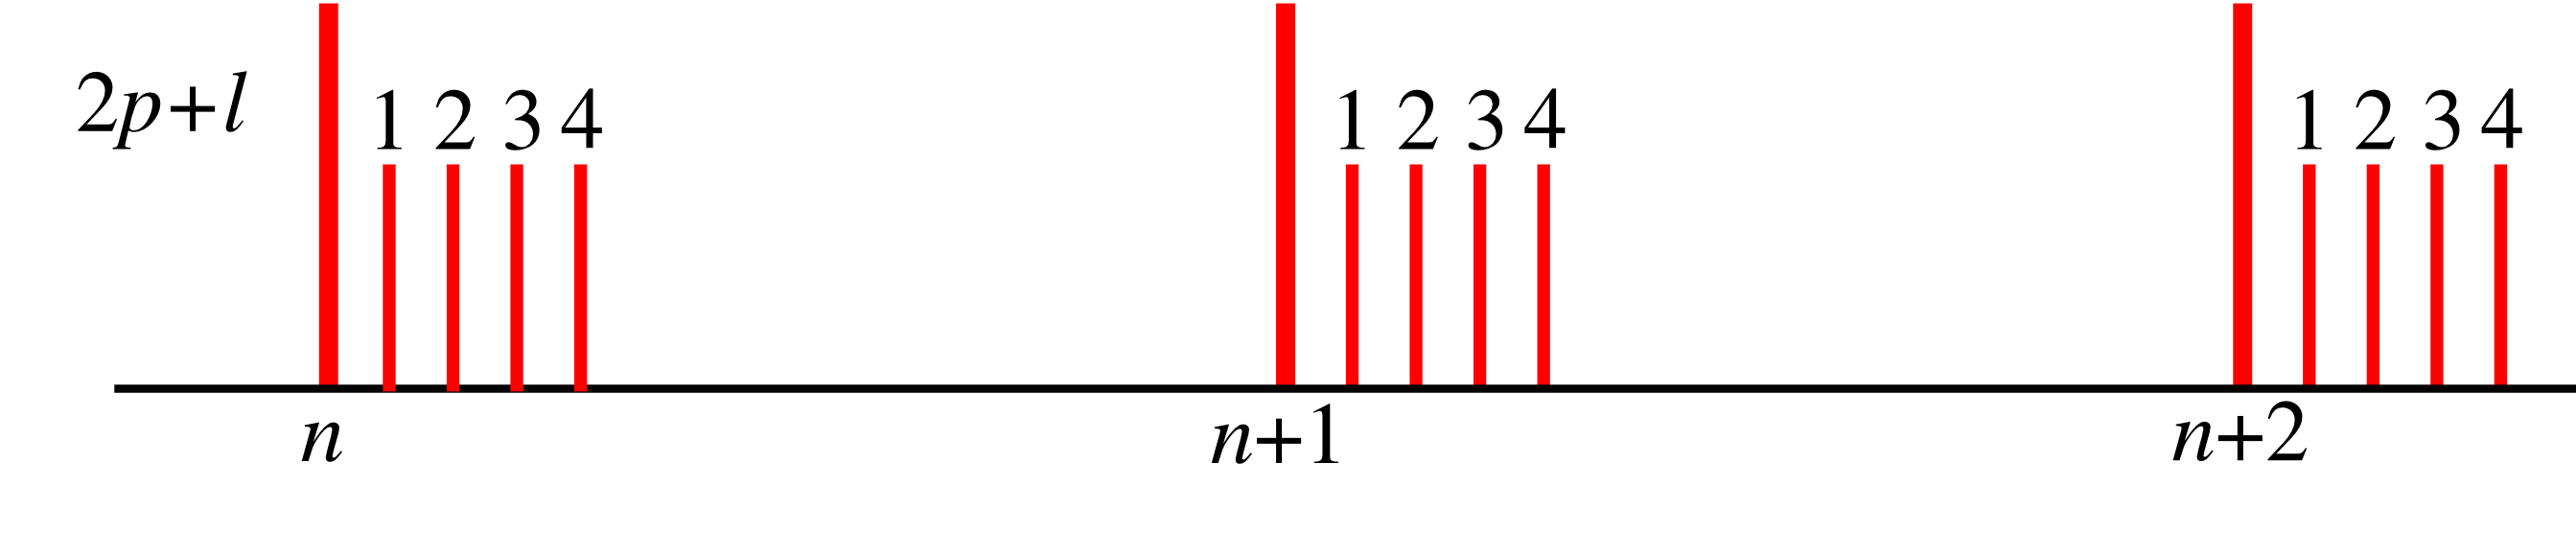
\includegraphics[width=10truecm]{slike/04_crte.png}
\caption{Resonančne frekvence za skoraj planparalelni ($R\gg L$) resonator.}
\label{fig:crte}
\end{figure}

\section{Izgube v resonatorjih}
Energija lastnega nihanja odprtega resonatorja ni konstantna, ampak se počasi
zmanjšuje zaradi več vzrokov:\\
\begin{enumerate}
\item Odbojnost ogledal ni enaka 1. Tudi če bi znali narediti popolno odbojna zrcala, 
tak resonator ne bi bil uporaben, saj nihanja ne bi mogli sklopiti z zunanjim poljem. Če 
torej hočemo dobiti nekaj svetlobe iz laserja ali filtrirati vpadajoči
snop, mora biti odbojnost zrcal manjša od 1.\\
\item Na sredstvu in na optičnih elementih v resonatorju pride do absorpcije in
sipanja svetlobe. Te izgube želimo navadno čim bolj zmanjšati.\\
\item Uklonske izgube so odvisne od premera zrcal in premera snopa na njih.
V dani geometriji imajo najmanjši polmer osnovni snopi, snopi višjega
reda so širši, zato imajo večje uklonske izgube. Merilo za uklonske
izgube je Fresnelovo število\index{Fresnelovo število} (enačba~\ref{eq:Fresnelovo_stevilo}) 
$N_{F}=a^{2}/(L\lambda)$, kjer je $a$ polmer ogledal. Pri enakem $N_{F}$ je
polmer snopa na izhodnem zrcalu najmanjši, če je resonator konfokalni\index{Resonator!konfokalni}, 
zato ima tak resonator tudi najmanjše uklonske izgube (glej nalogo~\ref{naloga:uklon_konf}).
Če je $N_{F}$ znatno večji od 1, kar navadno je, so uklonske izgube zanemarljive. \\
\end{enumerate}

Vse izgube lahko popišemo z razpadnim časom za energijo nihanja 
\begin{equation}
\frac{dW}{dt}=-\frac{2}{\tau}W \quad \textrm{in} \quad W = W_0 e^{\frac{-2t}{\tau}},
\label{eq:dW}
\end{equation}
pri čemer $\tau$ imenujemo življenjski čas nihanj\index{Življenjski čas nihanj}.
Izguba energije na en obhod resonatorja\index{Izgube v resonatorju} je
\begin{equation}
-dW = (1-{\cal R}_{1})W+(1-{\cal R}_{2})W +\Lambda_{0} W = \Lambda W.
\label{eq:Lambda}
\end{equation}
S ${\cal R}_{1,2}$ smo označili odbojnosti zrcal, od katerih je navadno ena
kolikor mogoče blizu 1. Parameter $\Lambda_{0}$ popiše absorpcijo in
sipanje znotraj resonatorja ter morebitne uklonske izgube. Tipične vrednosti 
zanj so do nekaj stotink. Celotne izgube popišemo s parametrom $\Lambda$. 

Razpadni čas nihanja lahko neposredno povežemo z izgubami, če v enačbo~(\ref{eq:dW})
vstavimo čas enega obhoda $t=2L/c$. Dobimo
\beq
\frac{dW}{W}= \Lambda = -\frac{2}{\tau}\, \frac{2L}{c},
\eeq
od koder sledi
\beq
\frac{1}{\tau}=\frac{\Lambda c}{4L}=\frac{1}{\tau_{0}}+\frac{c}{4L}[(1-{\cal R}_{1})+(1-{\cal R}_{2})],
\label{taulambda}
\eeq
kjer smo s $\tau_{0}=\Lambda_{0}\frac{c}{4L}$ označili razpadni
čas zaradi notranjih izgub. Notranje izgube so navadno zelo majhne, odbojnost enega zrcala
pa je približno enaka 1, tako da dobimo za življenjski čas nihanj 
\boxeq{eq:taucca}{
\frac{1}{\tau}=\frac{c}{4L} (1-{\cal R}).
}

Zaradi dušenja se energija lastnih nihanj eksponentno zmanjšuje, prav tako tudi
amplituda jakosti električnega polja. Amplituda pojema z dvakrat daljšim 
karakterističnim časom, ki je enak kar $\tau$. Spekter eksponentno pojemajoče funkcije izračunamo
(glej nalogo~\ref{naloga-spekter}) in dobimo Lorentzovo krivuljo s širino črte, ki ustreza ravno
\begin{equation}
\Delta\omega_{1/2}=\frac{1}{\tau}.
\label{3.26}
\end{equation}
Lastne frekvence torej niso neskončno ozke, ampak imajo končno širino $2/\tau$.
Poglejmo primer. Naj bodo notranje izgube na en obhod $\Lambda_0=0,01$,
eno zrcalo naj bo idealno, drugo naj ima ${\cal R}=0,93$. Dolžina
resonatorja naj bo $L=0,5$~m, valovna dolžina pa $500$~nm. Tedaj
je $1/\tau=12\cdot10^{6}$~s$^{-1}$. Zanimivo je pogledati razmerje med 
razmikom med zaporednima resonančnima frekvencama $\Delta \omega$ 
(enačba~\ref{eq:delta-omega-resonator}) in širino resonance $2/\tau$. 
Dobimo $\Delta\omega\tau/2 \approx 80$.\\

\begin{remark}
Namesto razpadnega časa $\tau$ se pogosto za opis izgub uporablja
dobrota resonatorja\index{Dobrota resonatorja}, ki jo vpeljemo kot
razmerje med resonančno frekvenco in širino črte 
\beq
Q=\frac{\omega_{n}}{\Delta\omega_{1/2}}.
\eeq
Za tipične optične resonatorje dobimo resonančno 
frekvenco $\omega_n \sim 10^{15}$~Hz, širino pa smo izračunali, da je reda 
 $1/\tau \sim 10^{7}$~Hz. Faktor dobrote je tako $Q \sim 10^{8}$. Optični 
 resonatorji imajo zelo velike faktorje dobrote!
\end{remark}

Poglejmo še primer, ko so notranje izgube zanemarljive in sta odbojnosti obeh zrcal enaki.
Potem dobimo iz enačbe~(\ref{taulambda})
\beq
\frac{1}{\tau}=\frac{c}{2L}(1-{\cal R}).
\eeq
Do istega rezultata pridemo tudi z razvojem izraza za prepustnost Fabry-Perotovega 
interferometra\index{Fabry-Perotov interferometer} (enačba~\ref{eq:Fabry-Perot-prepustnost})
okoli vrha pri $\omega_{n}$:
\begin{equation}
T=\frac{1}{1+\frac{4{\cal R}}{(1-{\cal R})^{2}}\sin^{2}L\frac{c}{(\omega-\omega_{n})}}\approx \frac{1}{1+\left[\frac{2}{(1-{\cal R})}\frac{L}{c}(\omega-\omega_{n})\right]^{2}},
\label{3.27}
\end{equation}
 kjer smo upoštevali še, da je odbojnost blizu ${\cal R} \approx 1$. Dobimo znano Lorentzovo
 krivuljo oblike
 \beq
 T = \frac{(\Delta\omega_{1/2})^2}{(\omega - \omega_n)^2+(\Delta\omega_{1/2})^2},
 \eeq
od koder hitro razberemo 
\beq
\frac{1}{\tau}=\Delta\omega_{1/2} = \frac{c}{2L}(1-{\cal R}).
\eeq

\section{*Obravnava z uklonskim integralom}
\label{Resonator_uklon}

V nestabilnih resonatorjih stacionarna rešitev v obliki stoječega
Gaussovega snopa ne obstoja. Poiskati rešitev za električno polje je
zato v takih resonatorjih precej zahtevno. 
Ker pa je problem soroden uklonu, ga lahko obravnavamo s pomočjo 
uklonske teorije.

Naj bo električno polje v točki $P_{1}$ prvega zrcala $E_{1}(P_{1})$.
Polje na drugem zrcalu lahko zapišemo s pomočjo Kirchhoffovega uklonskega
integrala\index{Kirchhoffov uklonski integral} (enačba~\ref{eq:Fresnelov-uklon})
\begin{eqnarray}
E_{2}(P_{2}) & = & -\frac{i}{2\lambda}\int_{1}E_{1}(P_{1})\frac{e^{ikr}(1+\cos\vartheta)}{r}\, dS_{1} \\
 & = & \int_{1}E_{1}(P_{1})K(P_{1},P_{2})dS_{1},
\label{eq:resuklon}
\end{eqnarray}
kjer je $r$ razdalja med točkama $P_{1}$ in $P_{2}$, $\vartheta$
je kot med zveznico in normalo na zrcala, druge faktorje pa smo pospravili v faktor
\beq
K(P_{1},P_{2}) = -\frac{i}{2\lambda}\frac{e^{ikr}(1+\cos\vartheta)}{r},
\label{jedro}
\eeq
ki predstavlja jedro integralske enačbe. Polje na prvem zrcalu mora
biti na enak način povezano s poljem na drugem. Če naj zapisano polje predstavlja lastno nihanje
resonatorja, mora biti po dveh odbojih sorazmerno začetnemu polju:
\begin{equation}
E_{1}(P)=-\gamma\int_{1}\int_{2}E_{1}(P_{1})K(P_{1},P_{2})K(P_{2},P_1)\, dS_{1}\, dS_{2}.
\label{3.71}
\end{equation}
Enačba~(\ref{3.71}) je homogena integralska enačba, katere lastne
rešitve so iskana lastna nihanja elektromagnetnega polja v resonatorju.
Kompleksne lastne vrednosti $\gamma$ določajo frekvenco in dušenje
nihanj. V splošnem rešitev ni mogoče poiskati analitično in se je
treba zateči k približnim numeričnim metodam. Najenostavnejša je iterativna
metoda, pri kateri začnemo z nekim začetnim poljem in ponavljamo integracijo
v enačbi~(\ref{3.71}), dokler se polje ne spreminja več.

Integralsko enačbo~(\ref{3.71}) je mogoče rešiti v posebnem primeru
konfokalnega resonatorja\index{Resonator!konfokalni}. Privzemimo, da je brez izgub. 
Ker je resonator simetričen, se polje na obeh zrcalih lahko razlikuje kvečjemu
za predznak.
\begin{figure}[h]
\centering
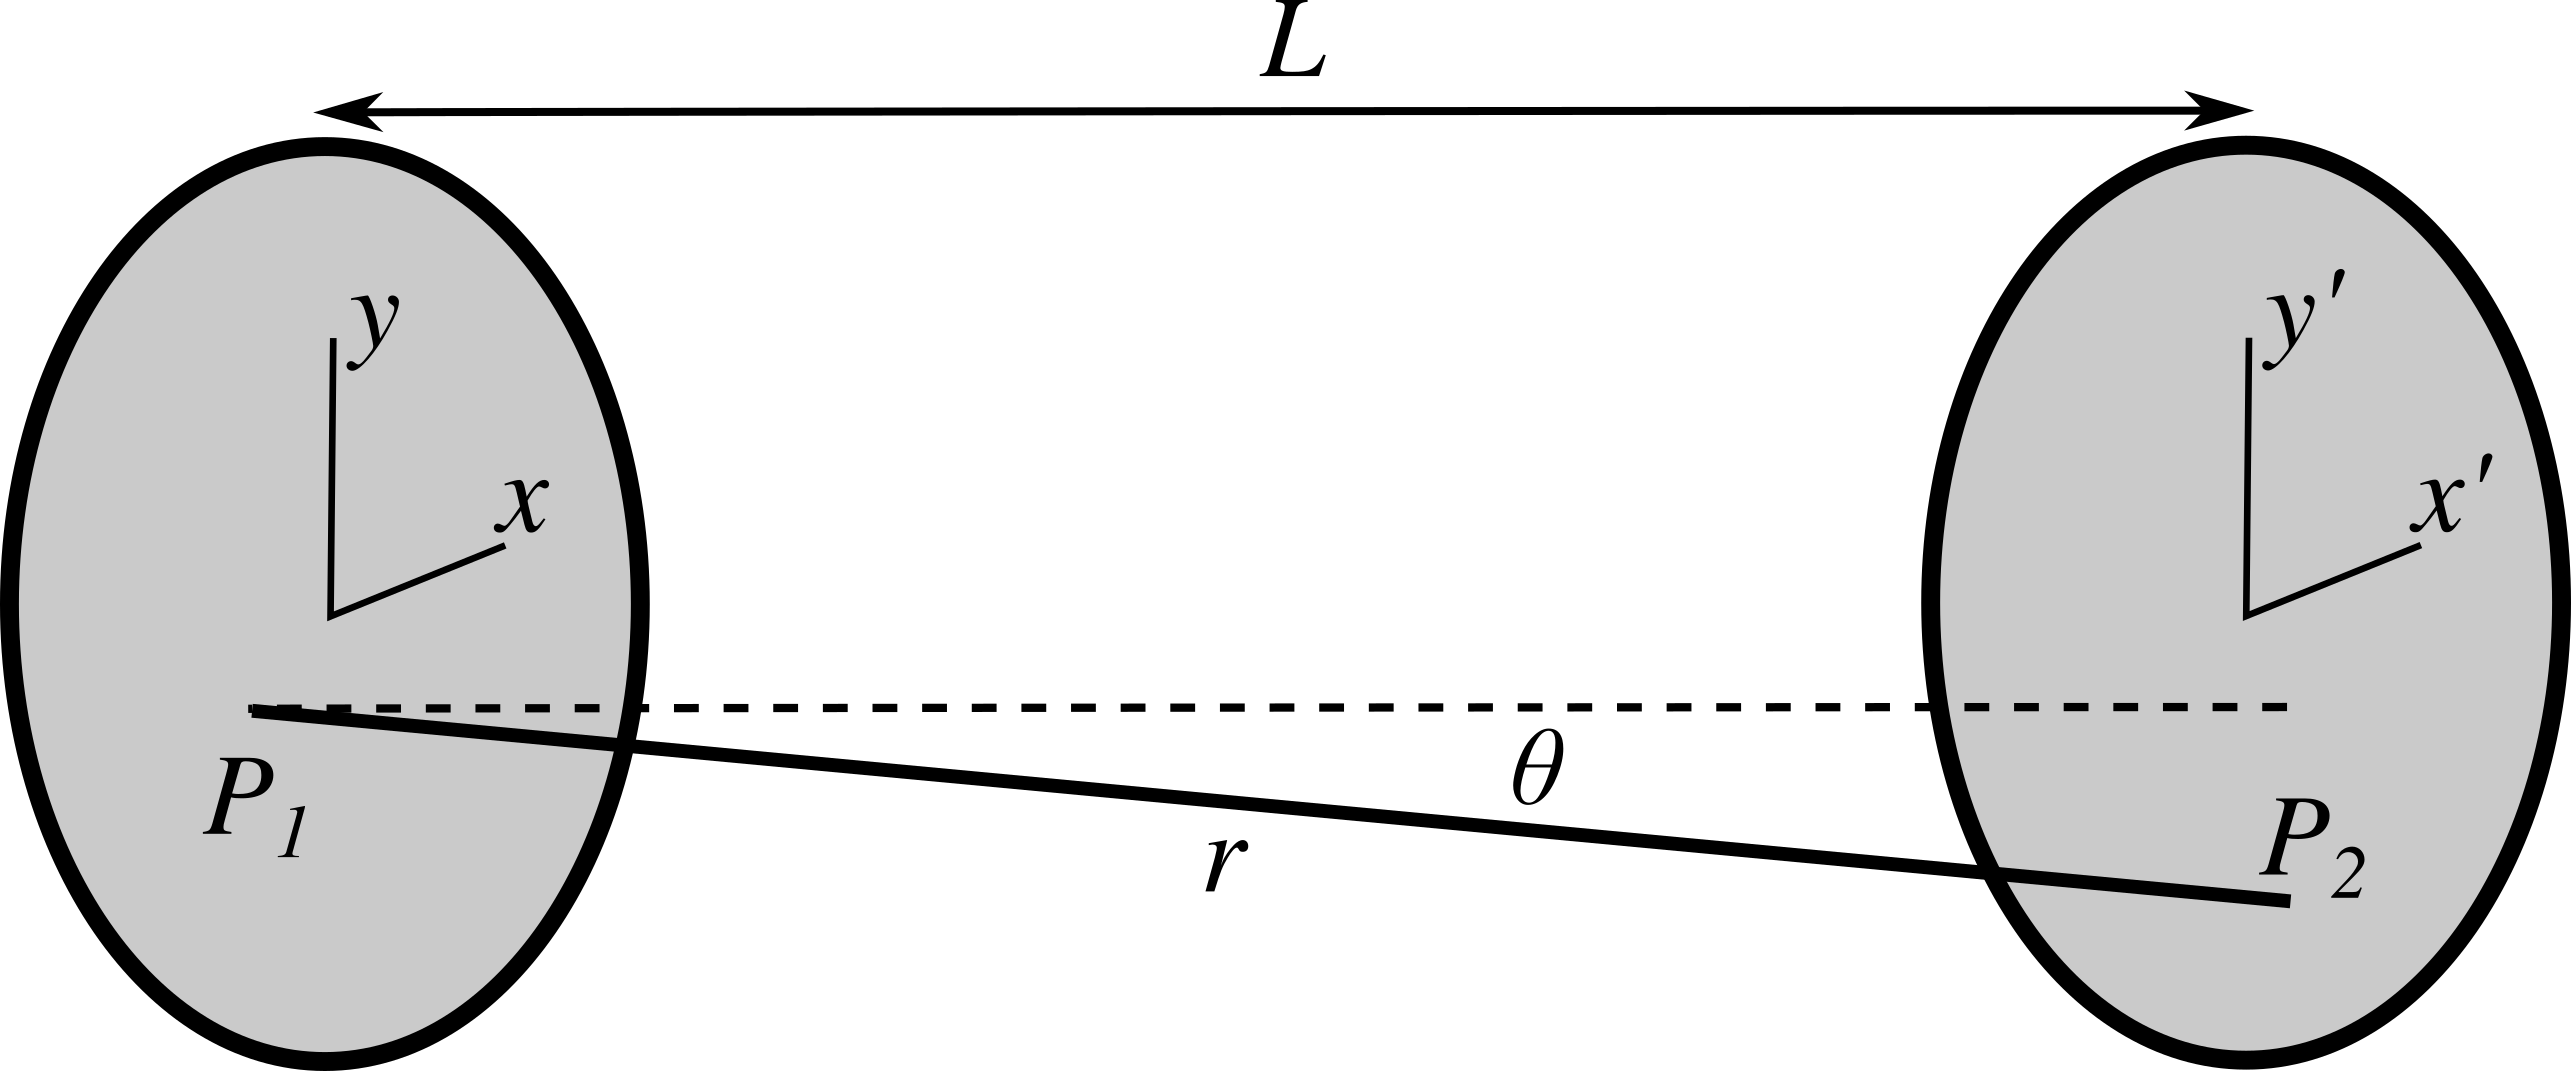
\includegraphics[width=7truecm]{slike/04_Uklon.png}
\caption{Koordinatna sistema na zrcalih resonatorja}
\label{fig:uklon_res_shema}
\end{figure}

Vpeljimo kartezične koordinate na obeh zrcalih, kot kaže slika~(\ref{fig:uklon_res_shema}).
Pričakujemo, da bo prečna razsežnost lastnega stanja majhna v primerjavi
z dolžino resonatorja, zato lahko $r$ razvijemo do drugega reda v
prečnih koordinatah
\begin{equation}
r\approx L-\frac{xx^{\prime}+yy^{\prime}}{L}.
\label{3.72}
\end{equation}
Ker obravnavamo konfokalni resonator, je krivinski radij zrcal kar enak dolžini resonatorja.
V imenovalcu jedra integrala (enačba~\ref{jedro}) zato lahko $r$ nadomestimo
z $L$. Koti med zveznico točk na obeh zrcalih in normalo na zrcali
so majhni, zato je  $\cos\vartheta \approx 1$. 

Tako iz enačbe~(\ref{eq:resuklon})
dobimo 
\begin{equation}
E(x',y')=\pm\frac{ie^{ikL}}{\lambda L}\int E(x,y)\exp
\left[\frac{-ik(xx^{\prime}+yy^{\prime})}{L}\right]\, dx\, dy.
\label{3.73}
\end{equation}
Integracija poteka po celem zrcalu. Jedro integrala je produkt dveh
faktorjev, ki vsebujeta vsak le $x'$ ali $y'$ koordinati. Zato poiščimo
rešitev enačbe~(\ref{3.73}) v obliki produkta 
\begin{equation}
E(x',y')=E_{0}f(x')g(y').
\label{3.74}
\end{equation}
S tem nastavkom morata biti funkciji $f(x')$ in $g(y')$ rešitve enačbe
\begin{equation}
\alpha f(x')=\int f(x)\exp\left[\frac{-ikxx^{\prime}}{L}\right]\, dx,
\label{3.75}
\end{equation}
kjer je $\alpha$ še neznana konstanta. Meje integrala so od enega do 
drugega roba zrcala. Če je dovolj veliko,
pričakujemo, da je polje na robu dovolj majhno, da lahko meje vzamemo
kar od $-\infty$ do $\infty$. Vpeljimo še brezdimenzijski koordinati
\begin{equation}
X'=x'\sqrt{k/L} \quad \mathrm{in} \quad Y'=y'\sqrt{k/L}.
\label{3.76}
\end{equation}
in dobimo
\begin{equation}
\alpha f(X')=\sqrt{\frac{L}{k}}\int_{-\infty}^{\infty}f(X)e^{-iXX^{\prime}}\, dX
\label{3.77}
\end{equation}
ter podobno enačbo za $g(Y')$. Enačba~(\ref{3.77}) pravi, da mora
biti $f(X)$ podobna svoji Fourierevi transformiranki. Najpreprostejša
funkcija s to lastnostjo je Gaussova funkcija 
\begin{equation}
f(X)=\exp[-\frac{1}{2}X^{2}].
\label{3.78}
\end{equation}
Polje na zrcalu ima tako po pričakovanju obliko Gaussovega snopa:
\begin{equation}
E(x,y)=E_{0}\exp\left[-\frac{k(x^{2}+y^{2})}{2L}\right].
\label{3.79}
\end{equation}

Poglejmo še konstanto $\alpha$. Imeti mora imeti vrednost 
$\alpha = \sqrt{2\pi L/k}=\sqrt{\lambda L}$.
Enaki izrazi veljajo tudi za smer $y$. Postavimo zdaj izračunano električno 
poljsko jakost (enačba~\ref{3.79}) z ustrezno vrednostjo za $\alpha$ v 
enačbo~(\ref{3.73}) in upoštevajmo, da mora biti
$E_{2}=\pm E_{1}$. Dobimo 
\begin{equation}
i\alpha^{2}\frac{e^{ikL}}{\lambda L}=ie^{ikL}=\pm1.
\label{3.80}
\end{equation}
Sledi že od prej poznani resonančni pogoj za
frekvenco lastnega stanja~(enačba~\ref{eq:omega_konf}):
\begin{equation}
\omega_{n}=ck_{n}=\frac{c}{L}(2n+1)\frac{\pi}{2}.
\label{3.81}
\end{equation}
Integralska enačba, dobljena iz uklonske teorije, tako da
isti rezultat kot stoječe valovanje oblike Gaussovih snopov, ki so
rešitve obosne valovne enačbe. To nas seveda ne preseneča, saj je
obosna valovna enačba enako natančna kot Fresnelova uklonska teorija.

\begin{definition}
Pokaži, da so funkcije, ki so sorazmerne svoji Fourierevi transformaciji, 
Hermite-Gaussove funkcije\index{Hermite-Gaussovi snopi} (enačba~\ref{eq:Gauss-Hermitevi}), in izračunaj lastne frekvence stanj višjega reda.
\end{definition}

\section{*Sklopitev resonatorja z okolico}
Na začetku poglavja smo omenili, da resonatorjev ne uporabljamo samo pri 
izdelavi laserjev, ampak lahko služijo tudi kot frekvenčni in
prostorski filtri za svetlobno valovanje. Povezavo med lastnimi nihanji
resonatorja in prepustnostjo ter odbojnostjo za valovanje, ki na resonator
vpada, bomo poiskali s formalizmom sklapljanja valovanj\index{Sklopitev valovanj}, 
ki je neke vrste perturbacijska analiza in je pogosto zelo uporaben.\\

Začnimo z resonatorjem z idealno odbojnimi stenami brez notranjih izgub. Stoječe
lastno valovanje v resonatorju zapišemo kot produkt krajevnega in časovnega
dela
\begin{equation}
E(\mathbf{r},t)=f(t)g(\mathbf{r}).
\label{3.31}
\end{equation}
Krajevni del $g(\mathbf{r})$ naj bo normaliziran tako, da je $\int g^{2}dV=1$. Iz valovne
enačbe (enačba~\ref{eq:valovna-skalarna}) sledi, da mora časovni del zadoščati 
nihajni enačbi drugega reda
\begin{equation}
\frac{\partial^2 f}{\partial t^2}+\omega_{n}^{2}f= \ddot{f} + \omega_{n}^{2}f=0.
\label{3.32}
\end{equation}
Vpeljemo lahko novo kompleksno spremenljivko $a$, ki je kombinacija funkcije $f$ in njenega
časovnega odvoda
\begin{equation}
a=\sqrt{\frac{\epsilon_{0}}{2}}(f+\frac{i}{\omega_{n}}\dot{f}).
\label{3.33}
\end{equation}
Izbira predfaktorja bo razvidna v nadaljevanju. 
Z odvajanjem in uporabo nihajne enačbe (enačba~\ref{3.32}) ugotovimo, da za $a$ velja 
preprosta diferencialna enačba 
\begin{equation}
\dot{a}=-i\omega_{n}a.
\label{3.34}
\end{equation}
Funkcija $a$ ima preprosto odvisnost od časa $e^{-i\omega_{n}t}$. \\

Zapišimo elektromagnetno energijo v resonatorju. Električni
del energije polja, ki je ravno polovica celotne energije, zapišemo kot
\beq
W_e = \frac{1}{2}\varepsilon_0 \int E^2 dV = \frac{1}{2}\epsilon_{0}f^{2}
\int g^{2}dV = \frac{1}{4} (a+a^{*})^2=\frac{1}{2}|a|^{2},
\eeq
\textcolor{red}{tako da je celotna energija lastnega nihanja resonatorja 
\begin{equation}
W=|a|^{2}.
\label{3.35}
\end{equation}}

Časovna odvisnost električnega polja $f(t)$ vsebuje člena z $e^{-i\omega_{n}t}$
in $e^{i\omega_{n}t}$, $a(t)$ pa ima le prvi člen. Zato ji včasih pravimo
tudi komponenta amplitude s pozitivno frekvenco. Prednost spremenljivke
$a$ je v enostavnejših enačbah, ki so le prvega reda. Spremenljivka $a$ in 
konjugirana spremenljivka $a^{*}$ sta tudi klasična oblika kreacijskih
in anihilacijskih operatorjev v kvantnomehanskem opisu harmonskega
oscilatorja.\\

Do zdaj smo obravnavali resonator brez izgub. Poglejmo si še primer z izgubami. 
Celotne izgube resonatorja lahko opišemo z dodatnim členom v enačbi~(\ref{3.34})
\begin{equation}
\dot{a}=-i\omega_{n}a-\frac{1}{\tau}a.
\label{3.36}
\end{equation}
V taki obliki lahko zapišemo enačbo le v primeru, če so izgube majhne. Če niso, 
je treba uporabiti navadno nihajno enačbo drugega reda. Gornji približek
namreč ne vsebuje zmanjšanja nihajne frekvence pri velikem dušenju.
Prehod na dve nesklopljeni enačbi prvega reda za $a$ in $a^*$
je točen le, kadar ni izgub. Izgube sklopijo enačbi za $a$ in $a^{\ast}$, 
vendar smo v našem približku to sklopitev zanemarili.

Naj bo odbojnost enega zrcala resonatorja nekoliko manjša od 1. Izgube v resonatorju 
se zato povečajo za (enačba~\ref{eq:taucca}) $1/\tau_{e}=c/(4L)(1-{\cal R})$. Druga posledica
zrcala z zmanjšano odbojnostjo pa je sklopitev resonatorja z okolico. To pomeni, 
da valovanje izhaja iz resonatorja, po drugi strani pa to pomeni tudi, da je 
lastno nihanje mogoče vzbujati z valovanjem, ki vpada na resonator.

Naj $s_{+}$ opiše snop valovanja, ki vpada na resonator. Amplituda $s_{+}$
naj bo izbrana tako, da je $|s_{+}|^{2}$ enako moči vpadnega valovanja. Zaenkrat
tudi izpustimo notranje izgube resonatorja $1/\tau_{0}$. Potem lahko
zapišemo 
\begin{equation}
\dot{a}=-i\omega_{n}a-\frac{1}{\tau_{e}}a+\kappa s_{+},
\label{3.37}
\end{equation}
kjer je $\kappa$ sklopitveni koeficient med vpadnim valovanjem in
amplitudo lastnega nihanja. Koeficient $\kappa$ je določen
s prepustnostjo zrcala, ki pa je vsebovana tudi v $1/\tau_{e}$. Koeficient
$\kappa$ torej ni neodvisen in poiščimo zvezo med $\kappa$ in $1/\tau_{e}$.

Naj ima vpadno valovanje frekvenco $\omega$. \textcolor{red}{Tedaj lahko iz enačbe~(\ref{3.37}) 
izračunamo amplitudo nihanja v stacionarnem stanju
\begin{equation}
a=\frac{\kappa s_{+}}{i(\omega_{n}-\omega)+1/\tau_{e}}.
\label{3.38}
\end{equation}
 }
Označimo zdaj del valovanja, ki se odbije ali izhaja od resonatorja, s $s_{-}$.
Če vpadnega vala ni, pojema energija nihanja zaradi odtekanja v $s_{-}$.
\textcolor{red}{Ohranitev energije da 
\begin{equation}
-\frac{dW}{dt}=-\frac{d}{dt}|a|^{2}=\frac{2}{\tau_{e}}|a|^{2}=|s_{-}|^{2}
\label{3.39}
\end{equation}
ali 
\begin{equation}
s_{-}=\sqrt{\frac{2}{\tau_{e}}}a,
\label{3.40}
\end{equation}
kjer smo fazo $s_{-}$ priredili z izbiro referenčne ravnine, v kateri
opazujemo $s_{-}$.}

Ob prisotnosti vpadnega vala $s_{+}$ lahko odbiti val zapišemo kot
vsoto direktnega odboja vpadnega vala $s_{+}$ in prispevka iz resonatorja
\begin{equation}
s_{-}=rs_{+}+\sqrt{\frac{2}{\tau_{e}}}a,
\label{3.41}
\end{equation}
kjer $r$ zaenkrat še ne poznamo. Ker ni notranjih izgub, mora bit v 
stacionarnem stanju vpadna moč enaka odbiti 
\begin{equation}
|s_{+}|^{2}=|s_{-}|^{2}.
\label{3.42}
\end{equation}
Uporabimo še izraz za stacionarno vrednost $a$  (enačba~\ref{3.38}) in dobimo
enakost 
\begin{equation}
r^{2}+\frac{2(\tau_{e}\kappa^{2}+r\kappa\sqrt{2\tau_{e}})}{1+\tau_{e}^{2}(\omega_{n}-\omega)^{2}}=1.\label{3.43}
\end{equation}
 Veljati mora pri vsaki frekvenci, to je pri vsaki vrednosti imenovalca
ulomka. Zato mora biti $r^{2}=1$ in $\tau_{e}\kappa=-r\sqrt{2\tau_{e}}$.
Ker sta $\tau_{e}$ in $\kappa$ pozitivna, je $r=-1$ in 
\begin{equation}
\kappa=\sqrt{\frac{2}{\tau_{e}}}\;\;.\label{3.44}
\end{equation}
 Odbito valovanje lahko torej zapišemo 
\begin{equation}
s_{-}=-s_{+}+\sqrt{\frac{2}{\tau_{e}}}a\;\;.\label{3.45}
\end{equation}

Z upoštevanjem notranjih izgub amplituda nihanja uboga enačbo 
\begin{equation}
\dot{a}=-i\omega_{n}a-(\frac{1}{\tau_{0}}+\frac{1}{\tau_{e}})a+\sqrt{\frac{2}{\tau_{e}}}s_{+}\;\;.\label{3.46}
\end{equation}
 Enačbi (\ref{3.45}) in (\ref{3.46}) sta osnovna izraza za sklaplanje
resonatorjev z enim vhodom. Za primer uporabe izračunajmo odbojnost
resonatorja $s_{-}/s_{+}$ kot funkcijo frekvence vpadnega vala. V
enačbo~(\ref{3.45}) postavimo izraz za stacionarno vrednost amplitude
nihanja 
\begin{equation}
a=\frac{\sqrt{\frac{2}{\tau_{e}}}s_{+}}{i(\omega_{n}-\omega)+(\frac{1}{\tau_{0}}+\frac{1}{\tau_{e}})}\label{3.47}
\end{equation}
 pa imamo 
\begin{equation}
\frac{s_{-}}{s_{+}}=\frac{\frac{1}{\tau_{0}}-\frac{1}{\tau_{e}}-i(\omega_{n}-\omega)}{\frac{1}{\tau_{0}}+\frac{1}{\tau_{e}}+i(\omega_{n}-\omega)}\;\;.\label{3.48}
\end{equation}
 Daleč od resonance je odbojnost -1. V resonanci, $\omega_{n}=\omega$,
odboja ni, kadar je $\tau_{e}=\tau_{0}$. Takarat je moč, ki gre iz
vpadnega valovanja v vzbujanje resonatorja, največja in je sklopitev,
ki jo meri $\tau_{e}$, popolnoma prilagojena izgubam. Taka prilagoditev
je analogna zahtevi, da mora biti impedanca bremena na koncu valovoda
ali koaksialnega kabla enaka impedanci valovoda oziroma kabla.

Če sta obe zrcali resonatorja delno prepustni, kot na primer pri običajnem
Fabri-Perotovem interferometru, bo enačba za amplitudo nihanja 
\begin{equation}
\dot{a}=-i\omega_{n}a-(\frac{1}{\tau_{0}}+\frac{1}{\tau_{e1}}+\frac{1}{\tau_{e2}})+\kappa_{1}s_{+1}+\kappa_{2}s_{+2}\;\;.\label{3.49}
\end{equation}
 $s_{+1}$ in $s_{+2}$ sta valovanji, ki vpadata z ene in druge strani.
Izgube zaradi končne prepustnosti so še vedno 
\begin{equation}
\frac{1}{\tau_{ei}}=\frac{c}{4L}(1-{\cal R}_{i})\;\;,\mbox{\hskip1cm}i=1,2\label{3.50}
\end{equation}
 S podobnim razmislekom kot prej, s tem da je najprej eno, nato drugo
vpadno valovanje nič, dobimo 
\begin{equation}
\kappa_{i}=\sqrt{\frac{2}{\tau_{ei}}}\;\;.\label{3.51}
\end{equation}
 Prepustnost resonatorja, to je razmerje med močjo vpadnega valovanja
z ene strani in izhodnega z druge, bo 
\begin{equation}
T=\frac{|s_{-2}|^{2}}{|s_{+1}|^{2}}=\frac{2}{\tau_{e2}}\frac{|a|^{2}}{|s_{+1}|^{2}}=\frac{4\tau^{2}/\tau_{e1}\tau_{e2}}{1+\tau^{2}(\omega_{n}-\omega)^{2}}\;\;,\label{3.52}
\end{equation}
 kjer je $1/\tau=1/\tau_{0}+1/\tau_{e1}+1/\tau_{e2}$. Če ni notranjih
izgub, je prepustnost v resonanci 
\begin{equation}
T=\frac{4/\tau_{e1}\tau_{e2}}{(1/\tau_{e1}+1/\tau_{e2})^{2}}\;\;.\label{3.53}
\end{equation}
 Prepustnost je v resonanci popolna, če sta obe zrcali enaki, $\tau_{e1}=\tau_{e2}$.
Gornja izraza se ujemata z znanim izrazom 
za prepustnost Fabri-Perotovega interferometra v bližini resonanc,
če so izgube in prepustnost zrcal majhne (enačba~\ref{eq:Fabry-Perot-prepustnost}).

Resonatorji imajo mnogo lastnih nihanj. Očitno veljajo gornji izrazi
za vsako posebej in dobimo celoten odziv resonatorja na poljubno vpadno
valovanje kot vsoto po vseh lastnih nihanjih. Pri tem ne smemo pozabiti,
da mora vpadno valovanje, ki se sklaplja z izbranim lastnim nihanjem,
imeti prostorsko odvisnost, ki ustreza lastnemu stanju. V primeru
stabilnih resonatorjev iz prejšnjih razdelkov mora torej biti vpadni
snop Gaussov z enakim $w_{0}$ in istega prečnega reda kot resonatorsko
stanje. Če vpadno valovanje ni tako, ga moramo najprej razviti po
Gaussovih snopih, ki ustrezajo resonatorju.

V praksi pri zahtevnejših interferometričnih meritvah je za to, da
vzbudimo le eno resonanco, potrebno vpadni snop prilagoditi resonatorju,
to je, polmer na vhodnem zrcalu mora biti enak polmeru lastnega nihanja,
krivinski radij vpadne valovne fronte pa enak krivinskemu radiju zrcala.
Obratno pa resonator deluje ne le kot frekvenčni filter, ampak tudi
kot prostorski. Recimo, da ima vpadno valovanje isto frekvenco kot
eno od nihanj resontorja. Prepuščeno valovanje bo imelo tedaj obliko
Gaussovega snopa, kot jo določa resonator, ne glede na obliko vpadnega
snopa.

Gornji način obravnave resonatorjev in sklopitve z vpadnim valovanjem
je posebej prikladen za račun nestacionarnega obnašanja in za primer,
ko je resonator napolnjen z nelinearnim sredstvom.


\section{*Sklopitev dveh resonatorjev}

\begin{figure}
 \caption{Resonatorja, sklopljena s polprepustnim zrcalom}


\label{sl3.5}\vskip7cm 
\end{figure}


Podobno kot sklopitev z zunanjim valovanjem lahko obravnavamo tudi
sklopitev med dvema resonatorjema. Imejmo dva resonatorja brez izgub,
sklopljena z delno prepustnim zrcalom, kot kaže slika (\ref{sl3.5}).
Sklopitev naj bo šibka, pa lahko zapišemo 
\begin{eqnarray}
\dot{a}_{1} & = & -i\omega_{1}a_{1}+\kappa_{12}a_{2}\nonumber \\
\dot{a}_{2} & = & -i\omega_{2}a_{2}+\kappa_{21}a_{1}\;\;.
\end{eqnarray}

Zaradi ohranitve energije sklopitvena koeficienta $\kappa_{12}$ in
$\kappa_{21}$ nista neodvisna. Vsota energij obeh resonatorjev mora
biti konstantna, zato 
\begin{eqnarray}
\frac{d}{dt}(|a_{1}|^{2}+|a_{2}|^{2}) & = & a_{1}\dot{a}_{1}^{*}+a_{1}^{*}\dot{a}_{1}+a_{2}\dot{a}_{2}^{*}+a_{2}^{*}\dot{a}_{2}\nonumber \\
 & = & a_{1}^{*}\kappa_{12}a_{2}+a_{1}\kappa_{12}^{*}a_{2}^{*}+a_{2}^{*}\kappa_{21}a_{1}+a_{2}\kappa_{21}^{*}a_{1}^{*}\nonumber \\
 & = & 0\;\;.
\end{eqnarray}
 Od tu vidimo, da mora biti 
\begin{equation}
\kappa_{12}+\kappa_{21}^{*}=0\;\;.\label{3.56}
\end{equation}

Za primer na sliki (\ref{sl3.5}) znamo sklopitveni koeficient brez
težav izračunati. V drugem resonatorju imamo stoječe valovanje. Moč
tistega dela, ki potuje proti prvemu resonatorju, je polovica energije,
deljena s časom preleta od enega zrcala do drugega: 
\begin{equation}
|s_{+}|^{2}=\frac{1}{2}|a_{2}|^{2}\frac{c}{L}\;\;.\label{3.57}
\end{equation}
 Z upoštevanjem enačbe (\ref{3.44}) je 
\begin{equation}
\kappa_{12}a_{2}=\sqrt{\frac{2}{\tau_{e}}}\, s_{+}=\sqrt{\frac{c}{\tau_{e}L}}\, a_{2}\;\;,\label{3.58}
\end{equation}
 tako da je 
\begin{equation}
\kappa_{12}=\frac{c}{2L}\sqrt{1-{\cal R}}\;\;,\mbox{\hskip1cm}\kappa_{21}=-\kappa_{12}\;\;.\label{3.59}
\end{equation}

Zaradi sklopitve se spremenijo lastne frekvence. Poglejmo dva enaka
sklopljena resonatorja: 
\begin{eqnarray}
\dot{a}_{1} & = & -i\omega_{0}a_{1}+\kappa_{12}a_{2}\nonumber \\
\dot{a}_{2} & = & -i\omega_{0}a_{2}-\kappa_{12}a_{1}\;\;.
\end{eqnarray}
 Iščemo rešitve oblike $A_{i}e^{-i\omega t}$. Če to postavimo v gornji
diferencialni enačbi, dobimo homogen linearen sistem za $A_{1}$ in
$A_{2}$, ki je netrivialno rešljiv, če je determinanta enaka nič.
To nam da enačbo za frekvenco 
\begin{equation}
(\omega-\omega_{0})^{2}=\kappa_{12}^{2}\label{3.61}
\end{equation}
 in 
\begin{equation}
\omega_{1,2}=\omega_{0}\pm\kappa_{12}\;\;.\label{3.62}
\end{equation}
 Zaradi sklopitve sta se prej enaki frekvenci razcepili v dve, kot
smo lahko pričakovali.
